\documentclass[]{scrbook}
\usepackage{lmodern}
\usepackage{amssymb,amsmath}
\usepackage{ifxetex,ifluatex}
\usepackage{fixltx2e} % provides \textsubscript
\ifnum 0\ifxetex 1\fi\ifluatex 1\fi=0 % if pdftex
  \usepackage[T1]{fontenc}
  \usepackage[utf8]{inputenc}
\else % if luatex or xelatex
  \ifxetex
    \usepackage{mathspec}
  \else
    \usepackage{fontspec}
  \fi
  \defaultfontfeatures{Ligatures=TeX,Scale=MatchLowercase}
\fi
% use upquote if available, for straight quotes in verbatim environments
\IfFileExists{upquote.sty}{\usepackage{upquote}}{}
% use microtype if available
\IfFileExists{microtype.sty}{%
\usepackage[]{microtype}
\UseMicrotypeSet[protrusion]{basicmath} % disable protrusion for tt fonts
}{}
\PassOptionsToPackage{hyphens}{url} % url is loaded by hyperref
\usepackage[unicode=true]{hyperref}
\hypersetup{
            pdftitle={Solver for Hydrologic Unstructured Domain (SHUD)},
            pdfauthor={Lele Shu (lele.shu@gmail.com)},
            pdfborder={0 0 0},
            breaklinks=true}
\urlstyle{same}  % don't use monospace font for urls
\usepackage{natbib}
\bibliographystyle{apalike}
\usepackage{longtable,booktabs}
% Fix footnotes in tables (requires footnote package)
\IfFileExists{footnote.sty}{\usepackage{footnote}\makesavenoteenv{long table}}{}
\usepackage{graphicx,grffile}
\makeatletter
\def\maxwidth{\ifdim\Gin@nat@width>\linewidth\linewidth\else\Gin@nat@width\fi}
\def\maxheight{\ifdim\Gin@nat@height>\textheight\textheight\else\Gin@nat@height\fi}
\makeatother
% Scale images if necessary, so that they will not overflow the page
% margins by default, and it is still possible to overwrite the defaults
% using explicit options in \includegraphics[width, height, ...]{}
\setkeys{Gin}{width=\maxwidth,height=\maxheight,keepaspectratio}
\IfFileExists{parskip.sty}{%
\usepackage{parskip}
}{% else
\setlength{\parindent}{0pt}
\setlength{\parskip}{6pt plus 2pt minus 1pt}
}
\setlength{\emergencystretch}{3em}  % prevent overfull lines
\providecommand{\tightlist}{%
  \setlength{\itemsep}{0pt}\setlength{\parskip}{0pt}}
\setcounter{secnumdepth}{5}
% Redefines (sub)paragraphs to behave more like sections
\ifx\paragraph\undefined\else
\let\oldparagraph\paragraph
\renewcommand{\paragraph}[1]{\oldparagraph{#1}\mbox{}}
\fi
\ifx\subparagraph\undefined\else
\let\oldsubparagraph\subparagraph
\renewcommand{\subparagraph}[1]{\oldsubparagraph{#1}\mbox{}}
\fi

% set default figure placement to htbp
\makeatletter
\def\fps@figure{htbp}
\makeatother

\usepackage{booktabs}

\title{Solver for Hydrologic Unstructured Domain (SHUD)}
\providecommand{\subtitle}[1]{}
\subtitle{User Guide}
\author{Lele Shu
(\href{mailto:lele.shu@gmail.com}{\nolinkurl{lele.shu@gmail.com}})}
\date{2019-11-23}

\begin{document}
\maketitle

{
\setcounter{tocdepth}{1}
\tableofcontents
}
\chapter{Overview}\label{Overview}

This is a user guide or technical documentation of the SHUD modeling
system.

The Solver for Hydrologic Unstructured Domain (SHUD - pronounced
``SHOULD'') is a multi-process, multi-scale hydrological model where
major hydrological processes are fully coupled using the semi-discrete
\textbf{Finite Volume Method} (FVM).

\textbf{SHUD-tools} is an open-source GIS and hydrological analysis
toolkit designed for SHUD modeling system. The SHUDtools provides access
to the digital data sets (terrain, forcing and parameters) and tools
necessary to drive the model, as well as a collection of GIS-based pre-
and post-processing tools.

Collectively the system is referred to as the \textbf{SHUD Modeling
System}.

The SHUD and SHUD-tools is an open source software, freely available for
download at \href{https://SHUD-system.github.io}{SHUD website} or
\href{https://github.com/SHUD-System/}{Github Page} along with
installation and user guides.

\section{Standing on the shoulder of
giant}\label{standing-on-the-shoulder-of-giant}

SHUD is a descendent of \textbf{Penn State Integrated Hydrologic Model
(PIHM)}, SHUD inherits the fundamental idea of solving hydrological
variables in CVODE, but the model structure, compurational algorithm,
programing laguage and input/out files are redesigned. The SHUD is
imcompatible to PIHM.

It is our intention (me and previous PIHM group)to begin a debate on the
role of \emph{Community Models} in the hydrologic sciences.

SHUD and PIHM represents our strategy for the synthesis of
\emph{multi-state}, \emph{multiscale} distributed hydrologic models
using the integral representation of the underlying physical process
equations and state variables.

Our interest is in devising a concise representation of watershed and/or
river basin hydrodynamics, which allows interactions among major
physical processes operating simultaneously, but with the flexibility to
add or eliminate states/processes/constitutive relations depending on
the objective of the numerical experiment or purpose of the scientific
or operational application.

To satisfy the objectives, the SHUD

\begin{itemize}
\tightlist
\item
  is distributed hydrologic model, based on the semi-discrete
  \textbf{Finite Volume Method (FVM)} in which domain discretization is
  an unstructured triangular irregular network (e.g.~Delaunay triangles)
  generated with constraints (geometric, and parametric). A local
  prismatic control volume is formed by the vertical projection of the
  Delaunay triangles forming each layer of the model. Given a set of
  constraints (e.g.~river network support, watershed boundary, altitude
  zones, ecological regions, hydraulic properties, climate zones, etc),
  an ``optimal'' mesh is generated. River volume elements are also
  prismatic, with trapezoidal or rectangular cross-section, and are
  generated along or cross edges of Delaunay triangles. The local
  control volume contains all equations to be solved and is referred to
  as the model kernel.
\item
  is a physically-based model, in which all equations used are
  describing the physics of the hydrological processes which control the
  catchment. The physical model is able to predict the water in the
  ungage water system, to estimate the sediment, pullutants, and
  vegetation, etc, such that it is practical to be coupled with
  biochemistry, geomorphology, limnology, and other water-related
  research. The global ODE system is assembled by combining all local
  ODE systems throughout the domain and then solved by a
  state-of-the-art parallel ODE solver known as CVODE developed at the
  Lawrence Livermore National Laboratory.
\item
  is a fully-coupled hydrologic model, where the state and flux
  variables in the hydrologic system are solved within the same time
  step and conserve the mass. The fluxes are infiltration, overland
  flow, groundwater recharge, lateral groundwater flow, exchange of
  river and soil/groundwater and river discharge.
\item
  is of an adaptable temporal and spatial resolution. The spatial
  resolution of the model varies from meters to kilometers based
  requirement of modeling and computing resources. The internal time
  step of the iteration step is adjustable; it is able to export the
  status of the catchment in less 1 second to days. Also, the time
  interval for exporting results is configured flexibly. The flexible
  spatial and temporal resolution is rather valuable for community model
  coupling.
\item
  is an open source model, anyone can access the source code, use and
  submit their improvement.
\item
  is a long-term yield and single-event flood model.
\end{itemize}

\section{Brief History of PIHM
system}\label{brief-history-of-pihm-system}

\begin{itemize}
\tightlist
\item
  2005 PIHM v1.0
\end{itemize}

Dr.~Yizhong Qu \citep{Qu2007} developed and verified the first version
of PIHM in 2001-2005 during his Ph.D.~in Pennsylvania State Unversity,
following the blueprint of Freeze and Harlan (1969). This version of
PIHM is the soul of the PIHM model.

\begin{itemize}
\tightlist
\item
  2009 PIHMgis
\end{itemize}

Dr.~Gopal Bhartt \citep{Bhatt2012} developed the PIHMgis with support of
C++, Qt GUI library, TRIANGLE library, and QGIS developing kit. The
development of PIHMgis makes the learning curve of PIHM moderate and
benefits the developing, modeling and coupling.

\begin{itemize}
\tightlist
\item
  2015 MM-PIHM
\end{itemize}

Dr.~Yuninh Shi led and developed the MM-PIHM (Multi-Module PIHM), which
embedded all modules from PIHM family, such as RT-PIHM, LE-PIHM,
flux-PIHM, BGC-PIHM, etc. together. The sophisticated design and
coupling of the MM-PIHM is the summit of the PIHM as a \emph{Community
Model} that combined all water-related modules together.

\begin{itemize}
\tightlist
\item
  2019 PIHM++
\end{itemize}

Based on the accumulated contribution of PIHM modeling and coupling with
related researches, it is necessary to solve the known bugs and
limitations, improve the performance of the model with parallel methods,
and adopt new updates from SUNDIALS solver and programming strategy.

Several publications that may helps:

\begin{itemize}
\tightlist
\item
  \citep{Qu2004}
\item
  \citep{Qu2007}
\item
  \citep{Li2008}
\item
  \citep{Kumar2004a}
\item
  \citep{Kumar2009d}
\item
  \citep{Yu2015}
\item
  \citep{Yu2014}
\item
  \citep{Li2011}
\item
  \citep{Shi2015}
\item
  \citep{Shi2015a}
\item
  \citep{Bhatt2014}
\end{itemize}

\section{Steps of modeling with SHUD}\label{steps-of-modeling-with-shud}

\subsection{Essential Terrestrial
Variables?}\label{essential-terrestrial-variables}

\begin{itemize}
\tightlist
\item
  Atmospheric forcing (precipitation, snow cover, wind, relative
  humidity, temperature, net radiation, albedo, photosynthetic
  atmospheric radiation, leaf area index)
\item
  Digital elevation model (DEM)
\item
  River/stream discharge
\item
  Soil (class, hydrologic properties)
\item
  Groundwater (levels, extent, hydro-geologic properties)
\item
  Lake/Reservoir (levels, extent)
\item
  Land cover and land use (biomass, human infrastructure, demography,
  ecosystem disturbance)
\item
  Water use
\end{itemize}

Most data reside on federal servers \ldots{}.many petabytes

\subsection{A-Priori Data Sources}\label{a-priori-data-sources}

\begin{longtable}[]{@{}ccc@{}}
\toprule
\begin{minipage}[b]{0.11\columnwidth}\centering\strut
Feature/Time-Series\strut
\end{minipage} & \begin{minipage}[b]{0.19\columnwidth}\centering\strut
Property\strut
\end{minipage} & \begin{minipage}[b]{0.42\columnwidth}\centering\strut
Source\strut
\end{minipage}\tabularnewline
\midrule
\endhead
\begin{minipage}[t]{0.11\columnwidth}\centering\strut
Soil\strut
\end{minipage} & \begin{minipage}[t]{0.19\columnwidth}\centering\strut
Porosity; Sand, Silt, Clay Fractions; Bulk Density\strut
\end{minipage} & \begin{minipage}[t]{0.42\columnwidth}\centering\strut
CONUS, SSURGO and STATSGO\strut
\end{minipage}\tabularnewline
\begin{minipage}[t]{0.11\columnwidth}\centering\strut
Geology\strut
\end{minipage} & \begin{minipage}[t]{0.19\columnwidth}\centering\strut
Bed Rock Depth; Horizontal and Vertical Hydraulic Conductivity\strut
\end{minipage} & \begin{minipage}[t]{0.42\columnwidth}\centering\strut
\url{http://www.dcnr.state.pa.us/topogeo/},
\url{http://www.lias.psu.edu/emsl/guides/X.html}\strut
\end{minipage}\tabularnewline
\begin{minipage}[t]{0.11\columnwidth}\centering\strut
Land Cover\strut
\end{minipage} & \begin{minipage}[t]{0.19\columnwidth}\centering\strut
LAI\strut
\end{minipage} & \begin{minipage}[t]{0.42\columnwidth}\centering\strut
\href{http://glcf.umiacs.umd.edu/data/landcover/data.shtml}{UMC},
\href{http://ldas.gsfc.nasa.gov/LDAS8th/MAPPED.VEG/LDASmapveg.shtml}{LDASmapveg};\strut
\end{minipage}\tabularnewline
\begin{minipage}[t]{0.11\columnwidth}\centering\strut
Land Cover\strut
\end{minipage} & \begin{minipage}[t]{0.19\columnwidth}\centering\strut
Manning's Roughness;\strut
\end{minipage} & \begin{minipage}[t]{0.42\columnwidth}\centering\strut
Hernandez et. al., 2000\strut
\end{minipage}\tabularnewline
\begin{minipage}[t]{0.11\columnwidth}\centering\strut
River\strut
\end{minipage} & \begin{minipage}[t]{0.19\columnwidth}\centering\strut
Manning's Roughness;\strut
\end{minipage} & \begin{minipage}[t]{0.42\columnwidth}\centering\strut
Dingman (2002)\strut
\end{minipage}\tabularnewline
\begin{minipage}[t]{0.11\columnwidth}\centering\strut
River\strut
\end{minipage} & \begin{minipage}[t]{0.19\columnwidth}\centering\strut
Coefficient of Discharge\strut
\end{minipage} & \begin{minipage}[t]{0.42\columnwidth}\centering\strut
ModHms Manual (Panday and Huyakorn, 2004)\strut
\end{minipage}\tabularnewline
\begin{minipage}[t]{0.11\columnwidth}\centering\strut
River\strut
\end{minipage} & \begin{minipage}[t]{0.19\columnwidth}\centering\strut
Shape and Dimensions;\strut
\end{minipage} & \begin{minipage}[t]{0.42\columnwidth}\centering\strut
Derived from regression using depth, width, and discharge data from
\href{http://nwis.waterdata.usgs.gov/usa/nwis/measurements}{USGS
data}\strut
\end{minipage}\tabularnewline
\begin{minipage}[t]{0.11\columnwidth}\centering\strut
River\strut
\end{minipage} & \begin{minipage}[t]{0.19\columnwidth}\centering\strut
Topology: Nodes, Neighboring Elements;\strut
\end{minipage} & \begin{minipage}[t]{0.42\columnwidth}\centering\strut
Derived using PIHMgis (Bhatt et. al., 2008)\strut
\end{minipage}\tabularnewline
\begin{minipage}[t]{0.11\columnwidth}\centering\strut
Forcing\strut
\end{minipage} & \begin{minipage}[t]{0.19\columnwidth}\centering\strut
Prec, Temp. RH, Wind, Rad.\strut
\end{minipage} & \begin{minipage}[t]{0.42\columnwidth}\centering\strut
National Land Data Assimilation System: NLDAS-2\strut
\end{minipage}\tabularnewline
\begin{minipage}[t]{0.11\columnwidth}\centering\strut
Topography\strut
\end{minipage} & \begin{minipage}[t]{0.19\columnwidth}\centering\strut
DEM\strut
\end{minipage} & \begin{minipage}[t]{0.42\columnwidth}\centering\strut
\url{http://seamless.usgs.gov/}\strut
\end{minipage}\tabularnewline
\begin{minipage}[t]{0.11\columnwidth}\centering\strut
Streamflow\strut
\end{minipage} & \begin{minipage}[t]{0.19\columnwidth}\centering\strut
\strut
\end{minipage} & \begin{minipage}[t]{0.42\columnwidth}\centering\strut
\url{http://nwis.waterdata.usgs.gov/nwis/sw}\strut
\end{minipage}\tabularnewline
\begin{minipage}[t]{0.11\columnwidth}\centering\strut
Groundwater\strut
\end{minipage} & \begin{minipage}[t]{0.19\columnwidth}\centering\strut
\strut
\end{minipage} & \begin{minipage}[t]{0.42\columnwidth}\centering\strut
\url{http://nwis.waterdata.usgs.gov/nwis/gw}\strut
\end{minipage}\tabularnewline
\bottomrule
\end{longtable}

\section{Workflow of SHUD Modeling
System}\label{workflow-of-shud-modeling-system}

\begin{figure}
\centering
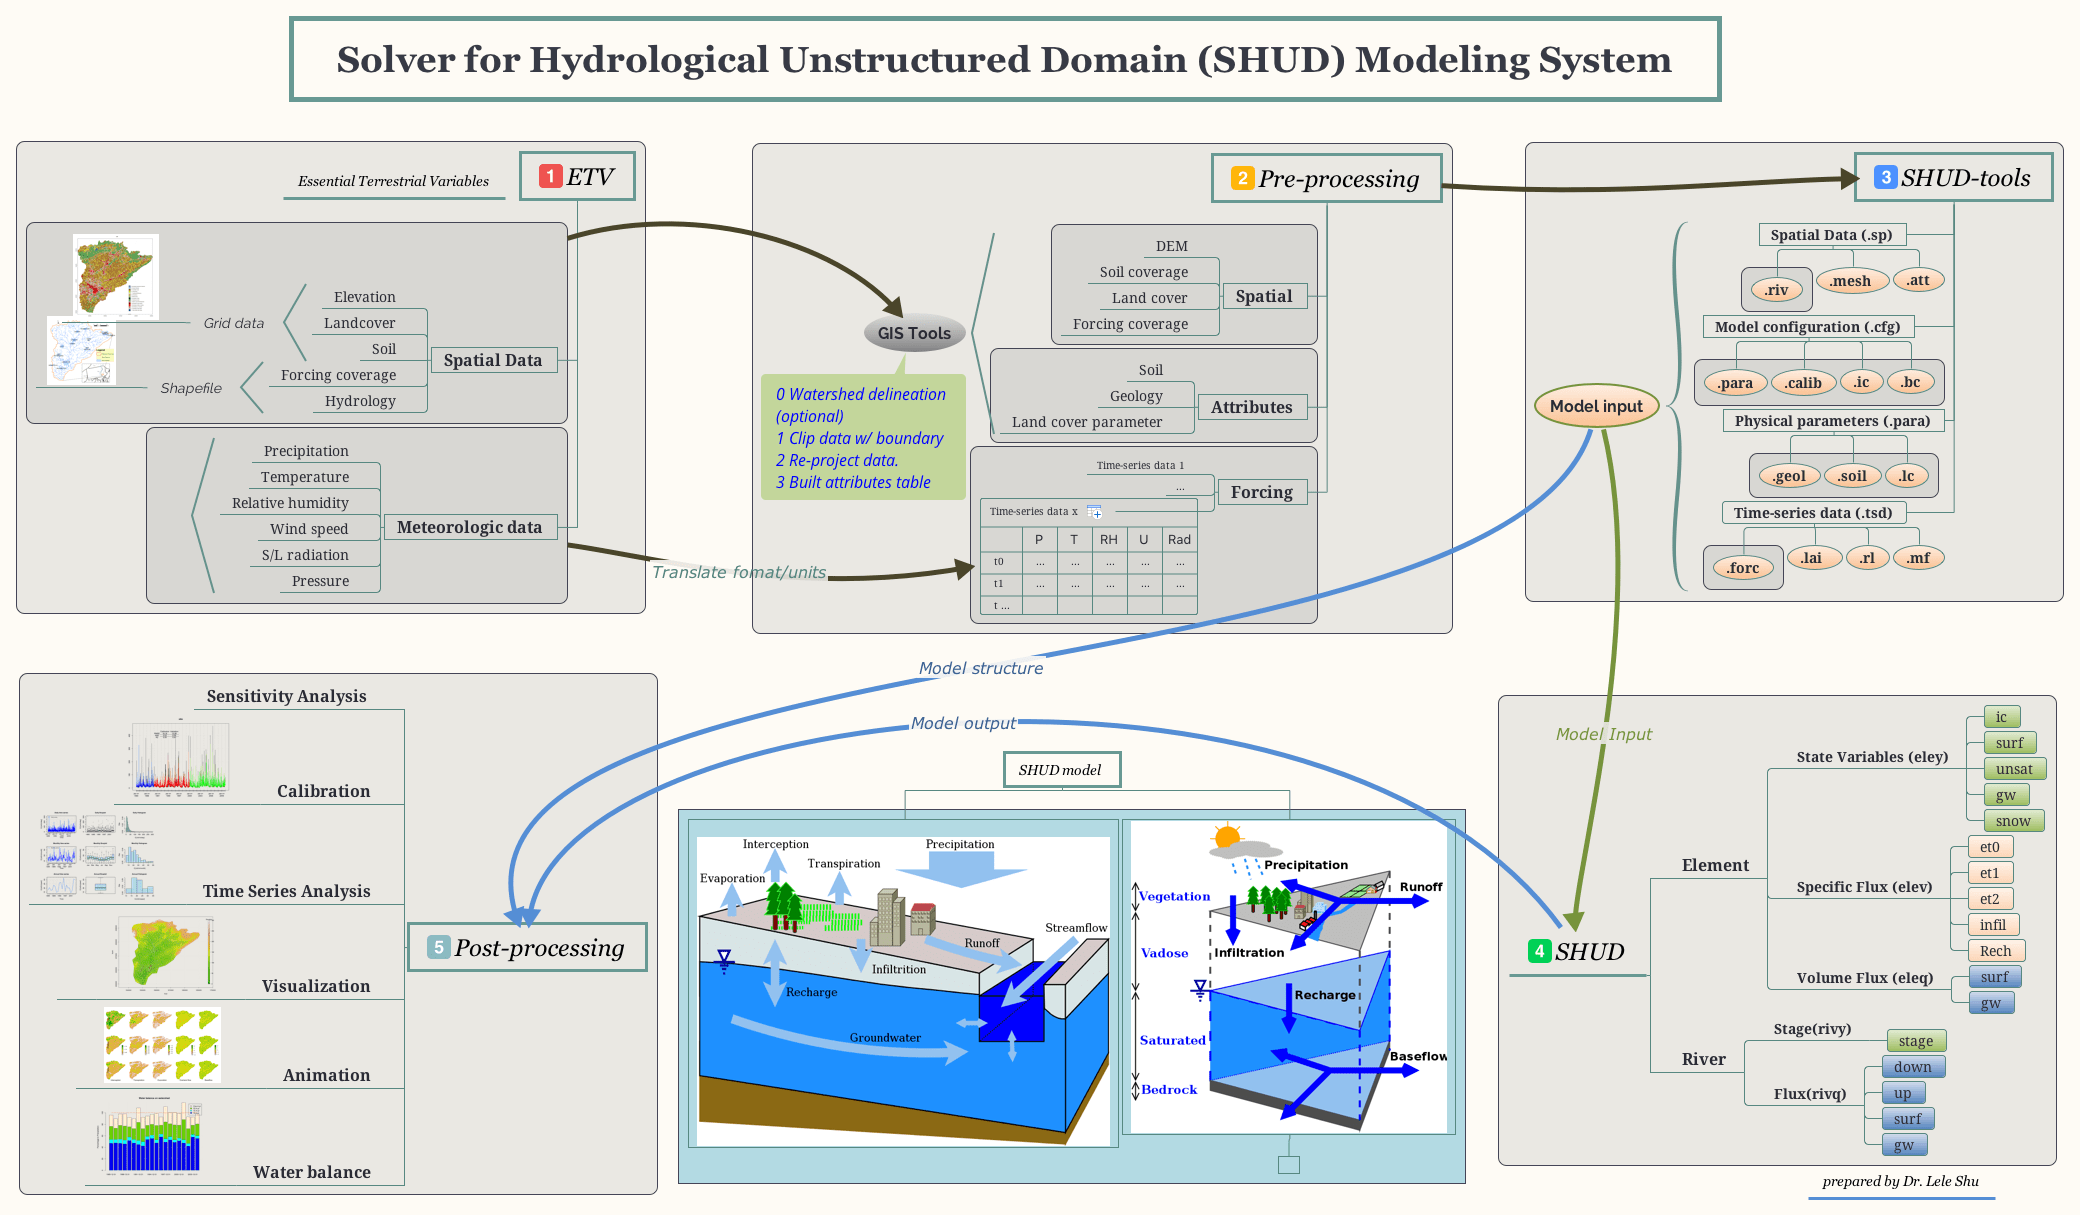
\includegraphics{./Fig/autoSHUD.png}
\caption{The workflow of modeling with SHUD Modeling System}
\end{figure}

\begin{enumerate}
\def\labelenumi{\arabic{enumi}.}
\tightlist
\item
  Prepare raw Essential Terrestrial Variables (ETV)
\item
  Convert and crop raw data with the research area boundary.
\item
  Build the unstructued modeling domain with
  \href{https://github.com/SHUD-System/SHUD-tools}{SHUD-tools}
\item
  Run SHUD on desktop or cluster.
\item
  Analysis the SHUD model results with
  \href{https://github.com/SHUD-System/SHUD-tools}{SHUD-tools} or your
  hydrologic analysis tools.
\end{enumerate}

\chapter{Install SHUD and SHUD-tools}\label{install-shud-and-shud-tools}

\section{SUNDIALS/CVODE}\label{sundialscvode}

The SHUD model requires the support of SUNDIALS or CVODE library.
\href{https://computation.llnl.gov/projects/sundials}{\textbf{SUNDIALS}}
is a SUite of Nonlinear and DIfferential/ALgebraic equation Solvers,
consists of six solvers.
\href{https://computation.llnl.gov/projects/sundials/cvode}{\textbf{CVODE}}
is a solver for stiff and nonstiff ordinary differential equation (ODE)
systems (initial value problem) given in explicit form \(y' = f(t,y)\).
The methods used in CVODE are variable-order, variable-step multistep
methods. You can install the entire SUNDIALS suite or CVODE only.

Since the SUNDIALS/CVODE keeps updating periodically and significantly,
the function names and structure are changed accordingly, we suggest to
use the specific version of the solver, rather than the latest solver.

SUNDIALS/CVODE is available in
\href{https://computation.llnl.gov/projects/sundials/sundials-software}{LLNL:
https://computation.llnl.gov/projects/sundials/sundials-software}

The installation of CVODE v3.x:

\begin{enumerate}
\def\labelenumi{\arabic{enumi}.}
\item
  Go to your Command Line and enter your workspace and unzip your CVODE
  source code here.
\item
  make directories for CVODE, including \emph{builddir}, \emph{instdir}
  and \emph{srcdir}

\begin{verbatim}
mkdir builddir
mkdir instdir
mkdir srcdir
cd builddir/
\end{verbatim}
\item
  Try ccmake. Install \texttt{cmake} if you don't have one.

\begin{verbatim}
ccmake 
\end{verbatim}
\item
  Run ccmake to configure your compile environment.

\begin{verbatim}
ccmake ../sundials/cvode-5.0.0
\end{verbatim}

  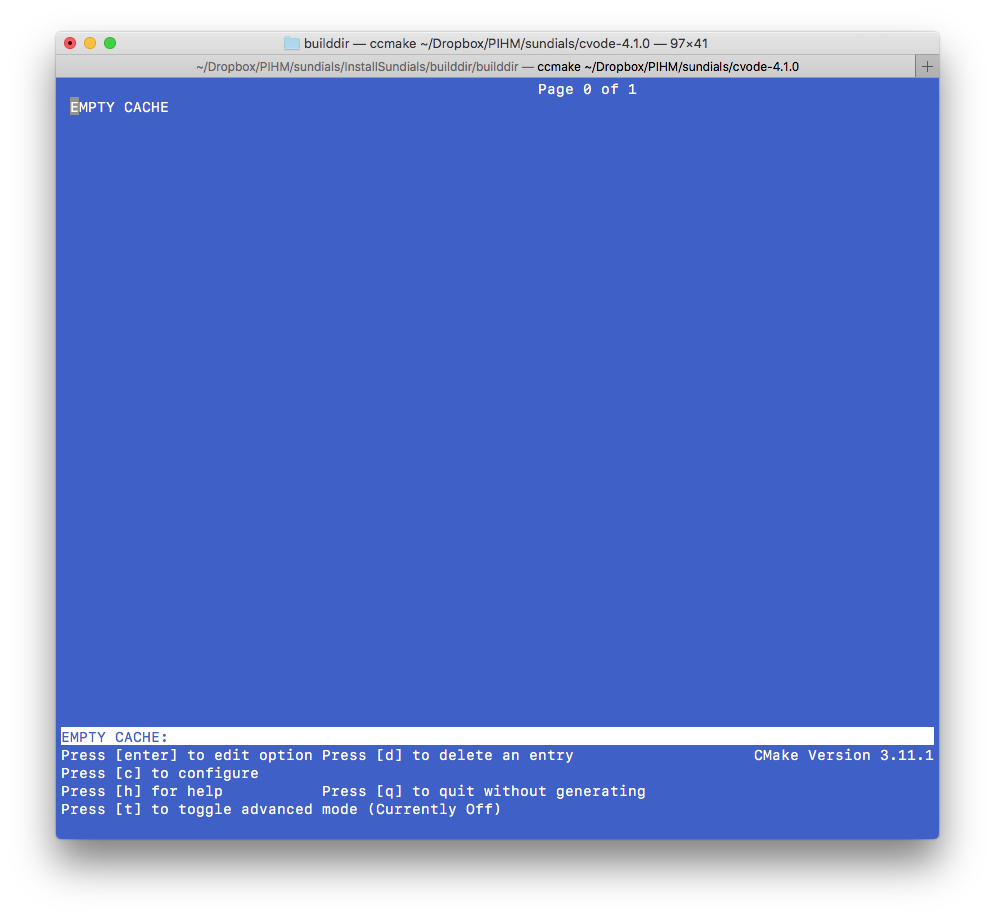
\includegraphics{Fig/ccmake/1.png} This is an empty configure. Press
  \texttt{c} to start the configuration.
\end{enumerate}

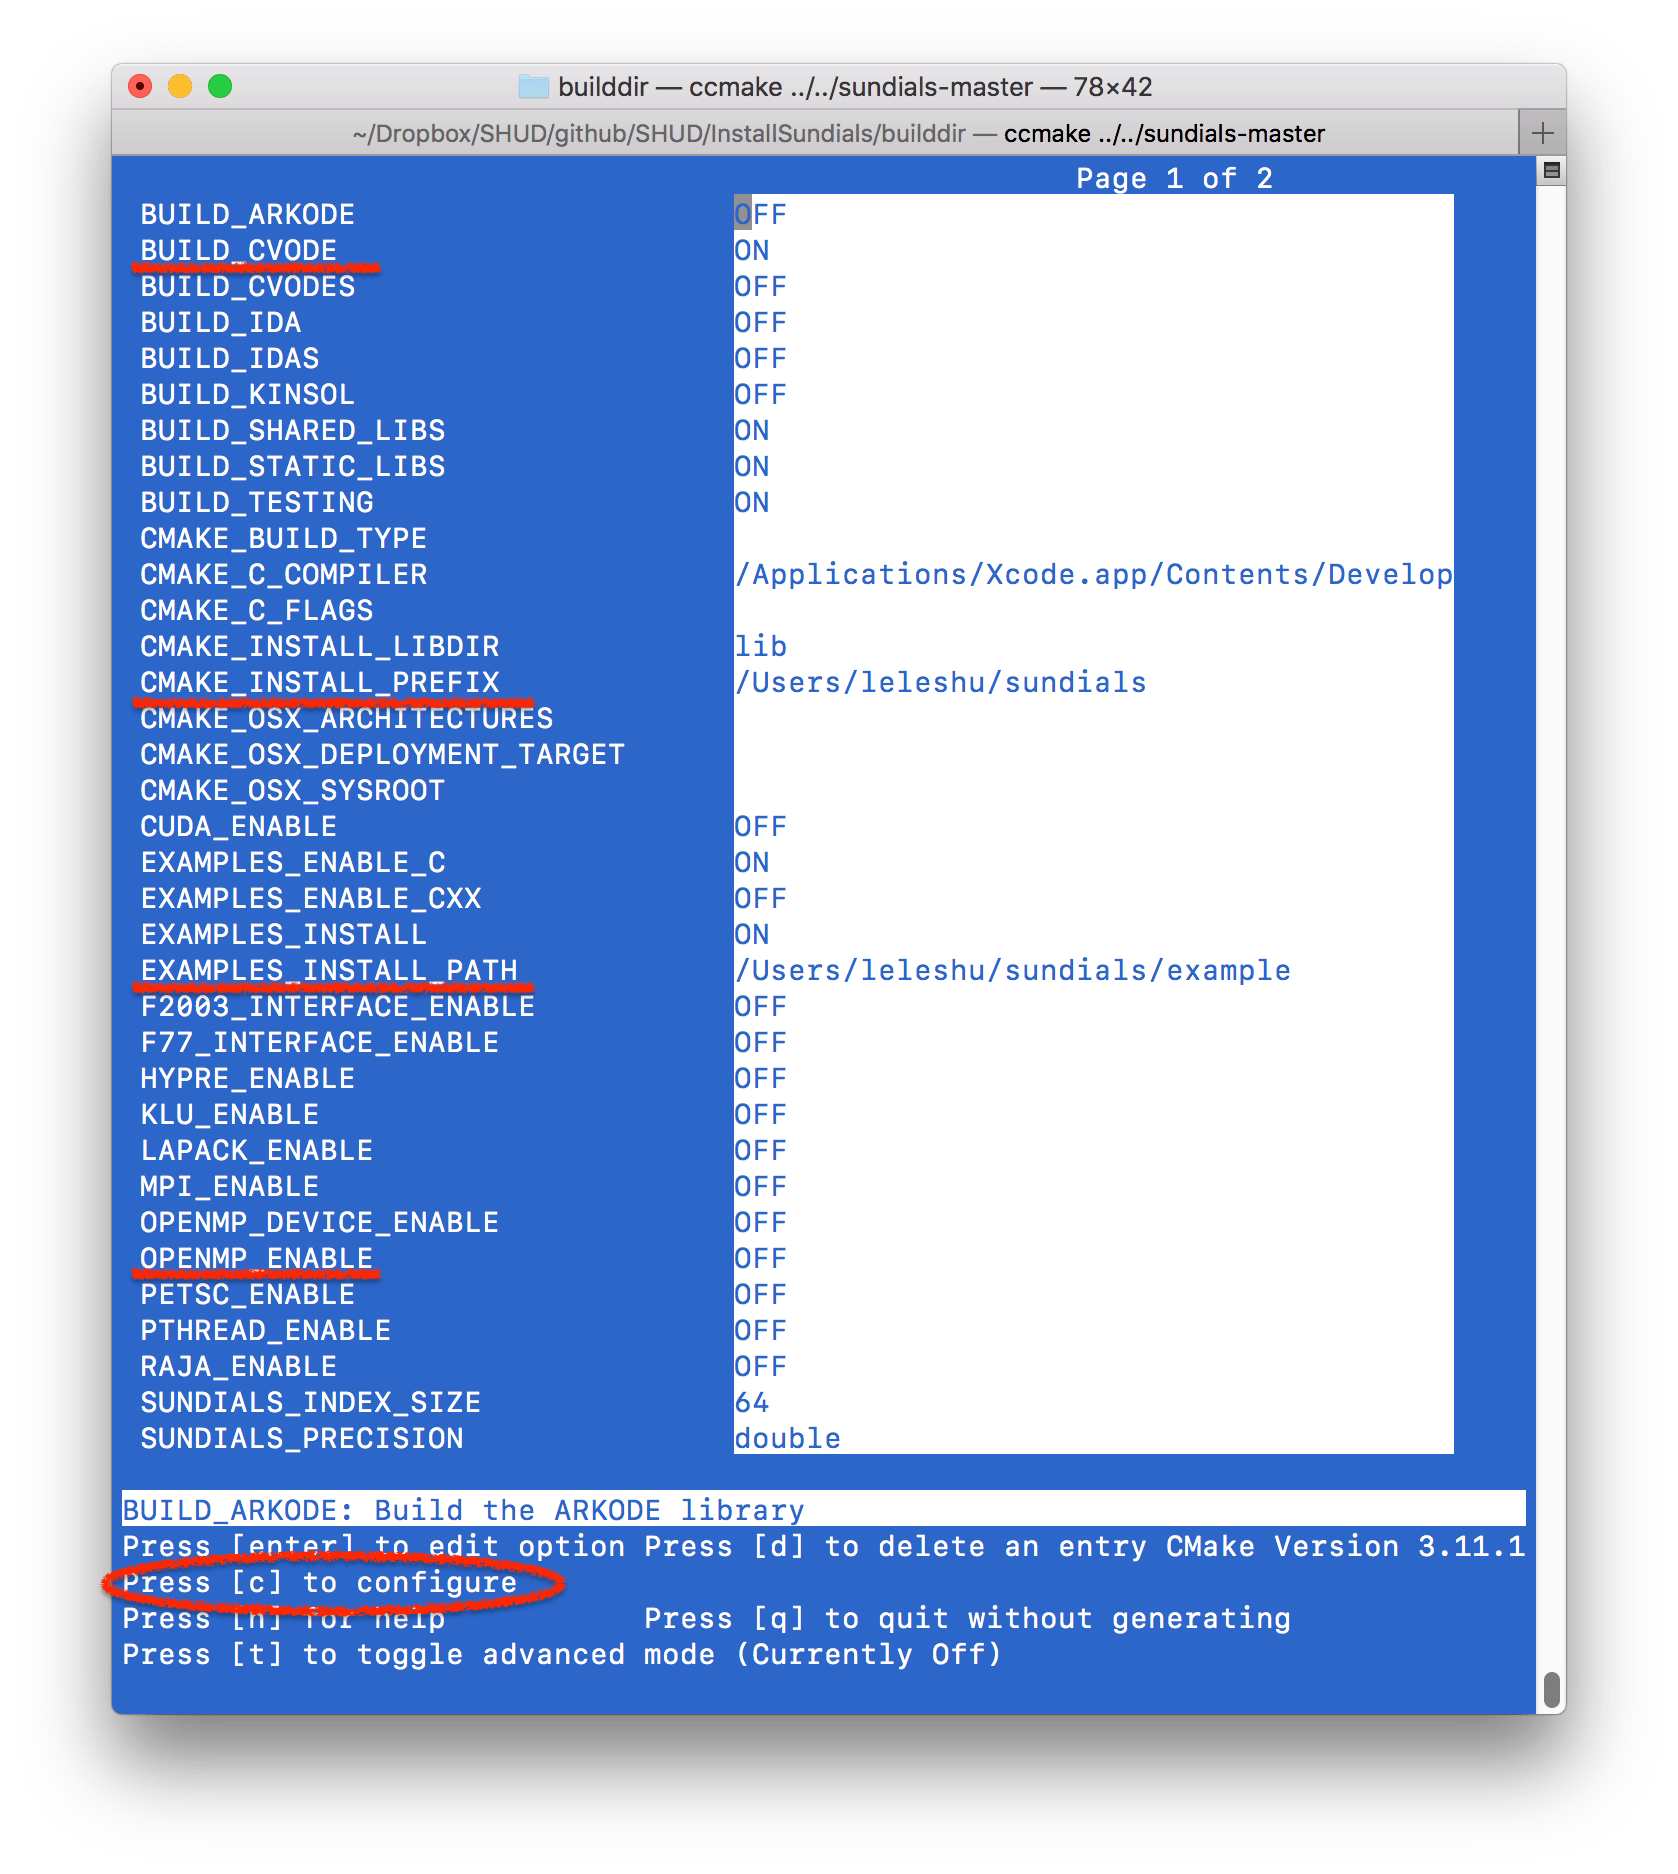
\includegraphics{Fig/ccmake/2.png} The default configuration. Make sure
the value for three lines:

\begin{verbatim}
BUILD_CVODE = ON
CMAKE_INSTALL_PREFIX = ~/sundials
EXAMPLES_INSTALL_PATH = ~/sundials/examples
\end{verbatim}

After the modification of values, press \texttt{c} to confirm
configuration.

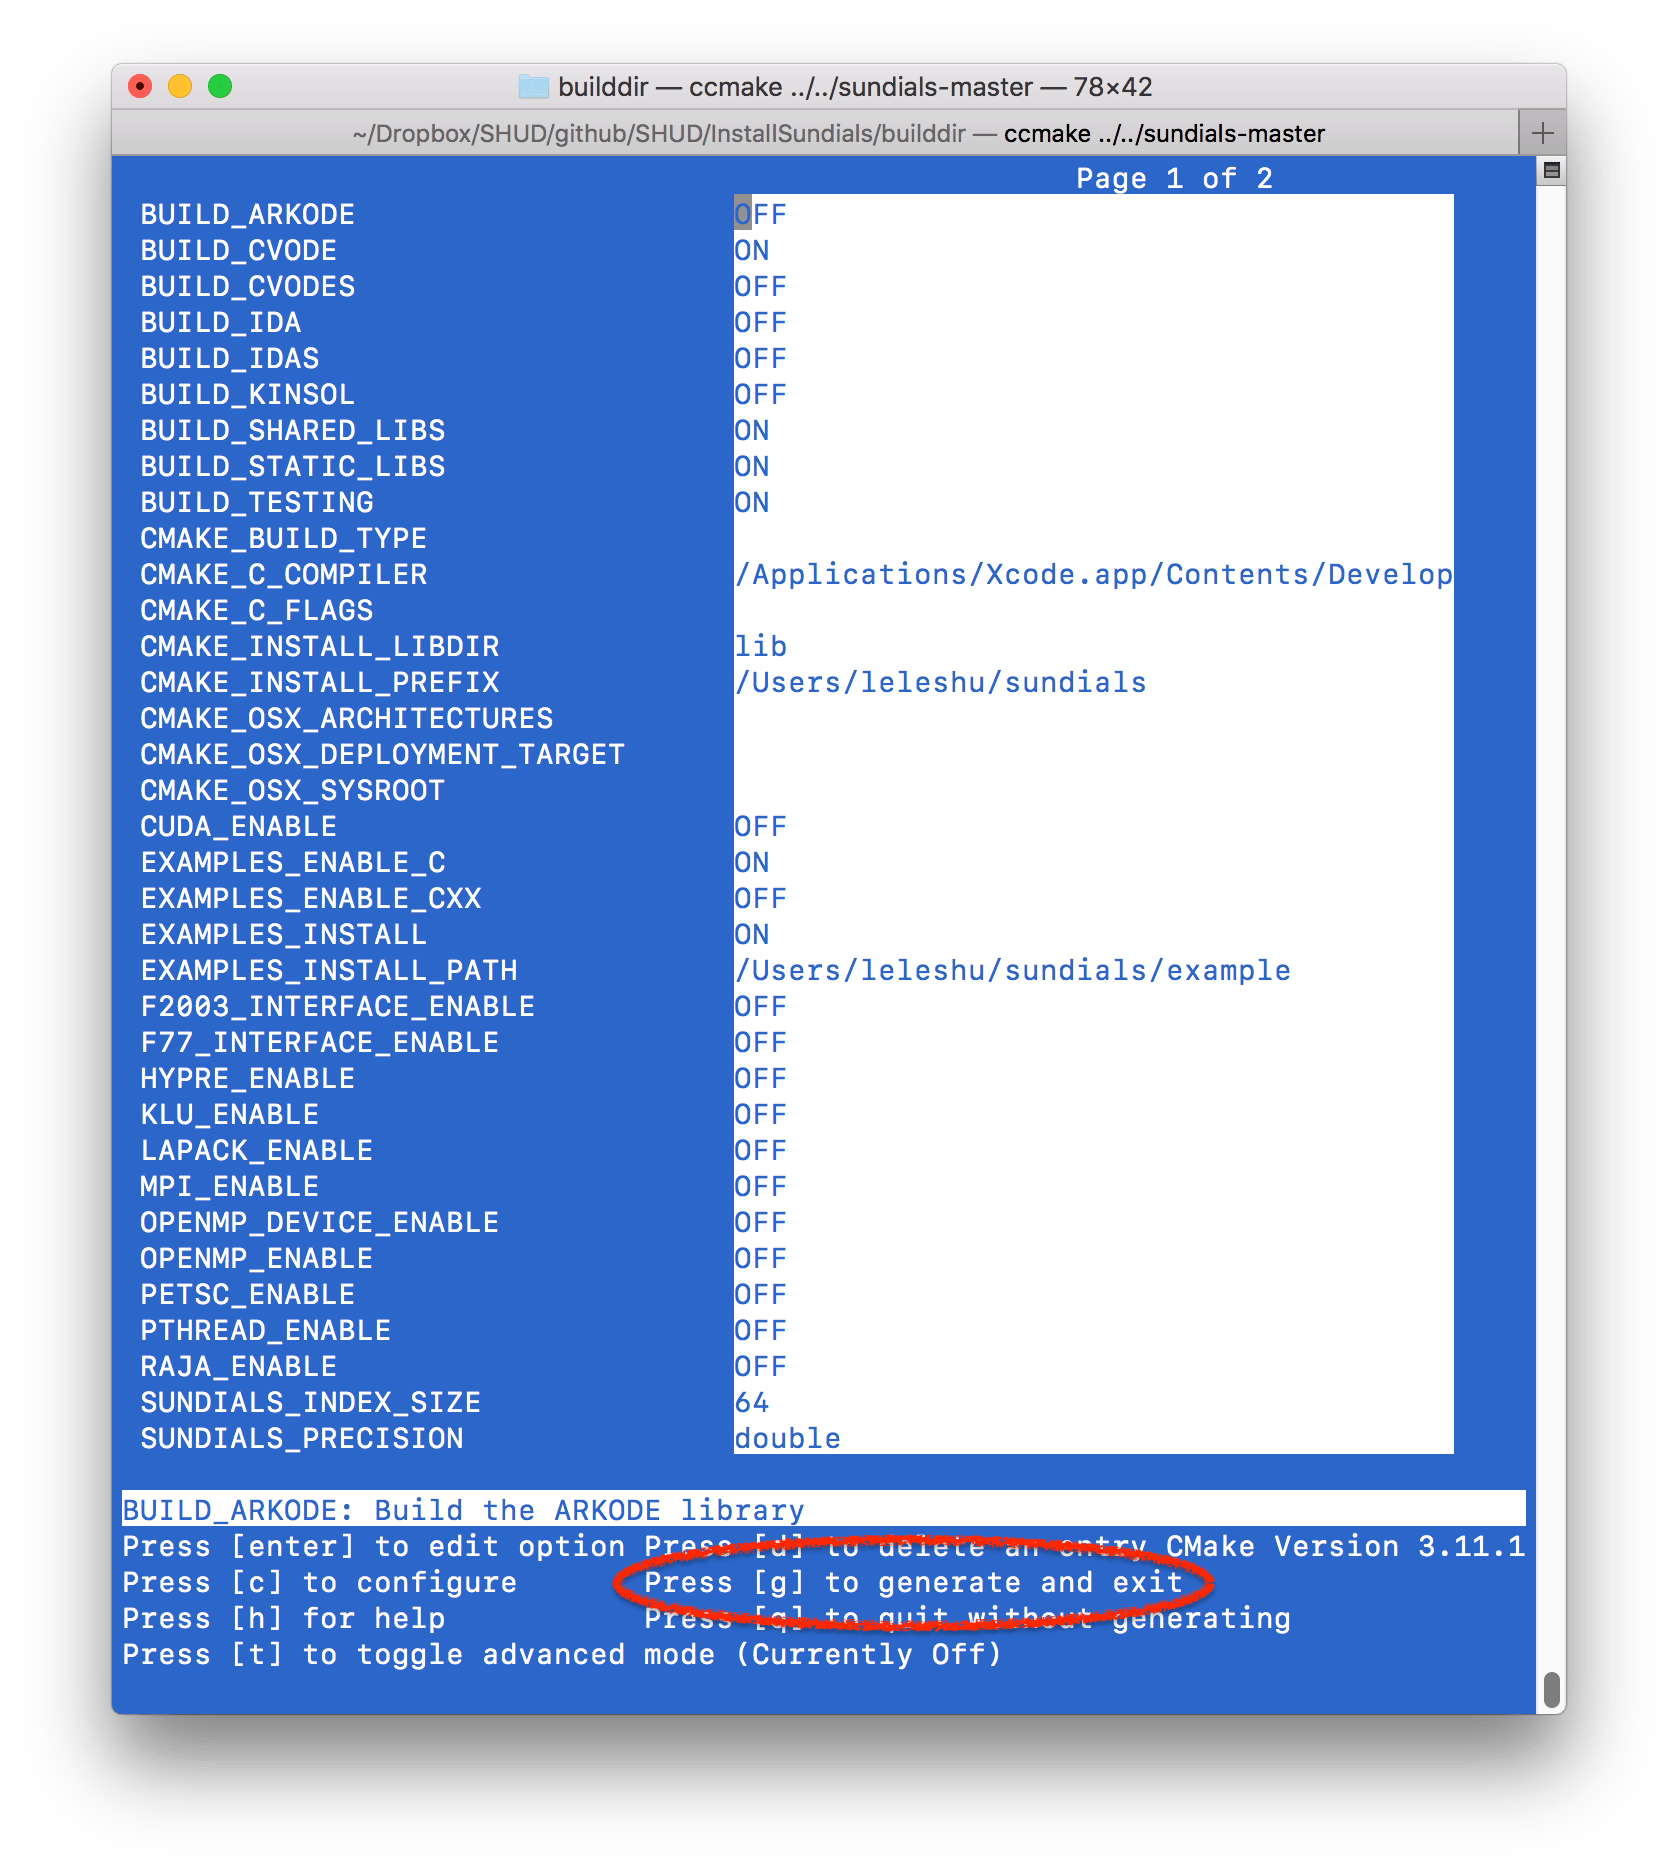
\includegraphics{Fig/ccmake/3.png} The ccmake configures the environment
automatically. When the configuration is ready, press \texttt{g} to
generate and exit.

\begin{enumerate}
\def\labelenumi{\arabic{enumi}.}
\item
  Then you run commands below:

\begin{verbatim}
make
make install 
\end{verbatim}
\end{enumerate}

\section{SHUD}\label{shud}

Configuration in \emph{Makefile}:

\begin{enumerate}
\def\labelenumi{\arabic{enumi}.}
\tightlist
\item
  Path of \emph{SUNDIALS\_DIR.} {[}\textbf{CRITICAL}{]}. If you install
  SUNDIALS into \emph{\textasciitilde{}/sundials}, you don't change this
  line..
\item
  Path of OpenMP if the parallel is preferred.
\item
  Path of SRC\_DIR, default is \texttt{SRC\_DIR\ =\ .}
\item
  Path of BUILT\_DIR, default is \texttt{BUILT\_DIR\ =\ .}
\end{enumerate}

After updating the SUNDIALS path in the \emph{Makefile}, user can
compile the SHUD with:

\begin{verbatim}
make clean
make shud
\end{verbatim}

There are more options to compile the SHUD code:

\begin{itemize}
\tightlist
\item
  \texttt{make\ all} - clean, then make both shud and shud\_omp
\item
  \texttt{make\ help} - help information
\item
  \texttt{make\ SHUD} - make SHUD executable
\item
  \texttt{make\ SHUD\_omp} - make shud\_omp with OpenMP support
\end{itemize}

\subsection{OpenMP}\label{openmp}

If parallel-computing is prefered, please install OpenMP. For mac:

\begin{verbatim}
brew install llvm clang
brew install libomp
compile flags for OpenMP: 
  -Xpreprocessor -fopenmp -lomp
Library/Include paths:
  -L/usr/local/opt/libomp/lib 
  -I/usr/local/opt/libomp/include
\end{verbatim}

\subsection{Run SHUD executables.}\label{run-shud-executables.}

After the successful installation and compile, you can run SHUD models
using

\begin{verbatim}
./shud <projectname>
\end{verbatim}

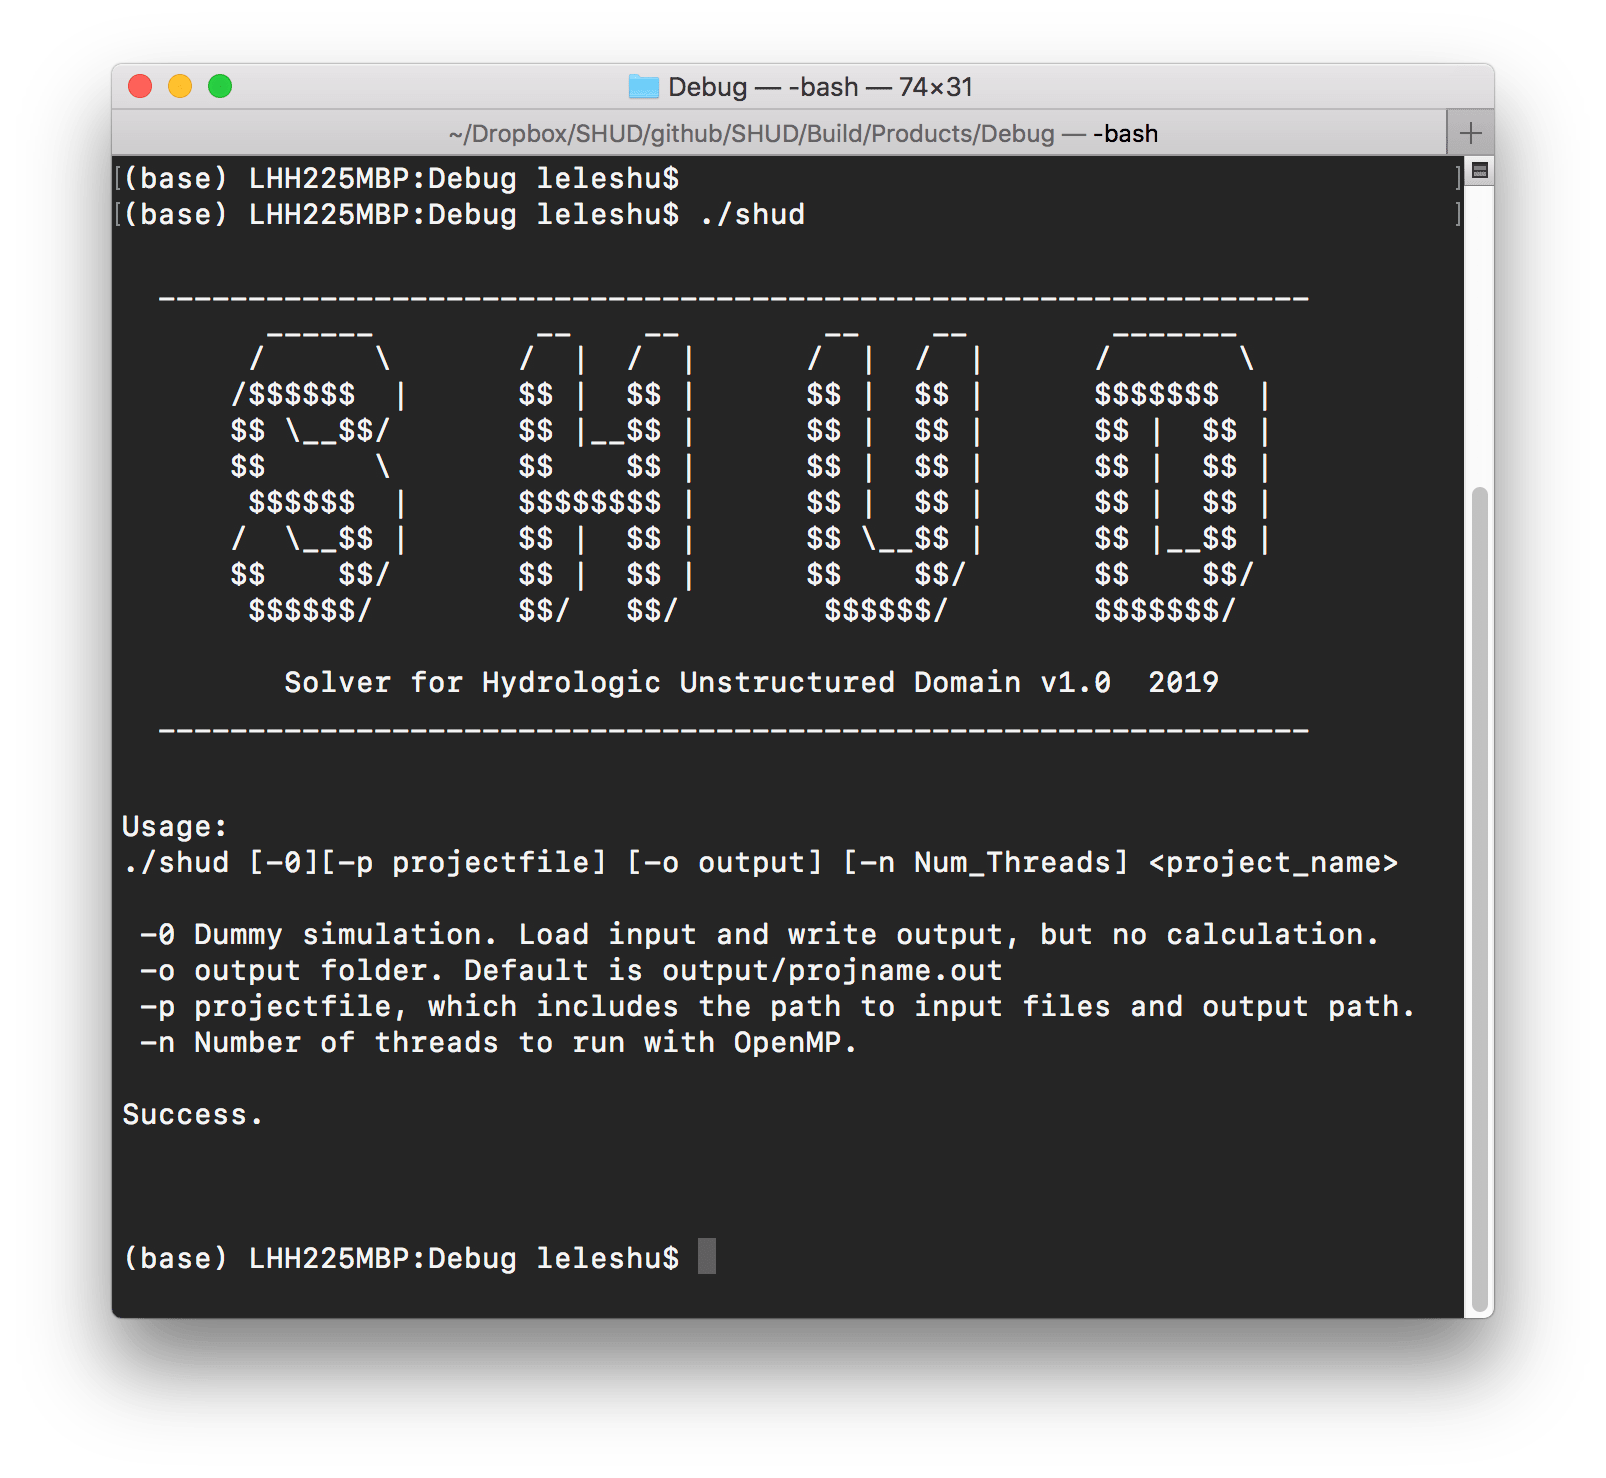
\includegraphics{Fig/CLI.png} Command line pattern is:

\begin{verbatim}
./shud [-0][-p projectfile] [-o output] [-n Num_Threads] <project_name>
\end{verbatim}

\begin{itemize}
\item
  \texttt{-0} Dummy simulation. Load input and write output, but no
  calculation.
\item
  \texttt{\textless{}project\ name\textgreater{}} is the name of the
  project.
\item
  \texttt{{[}-p\ projectfile{]}} Specify the project file, which
  includes the path to input files and output path.
\item
  \texttt{{[}-o\ output\_folder{]}} Output directory. Default is
  output/projname.out
\item
  \texttt{{[}-n\ Num\_Threads{]}} Number of threads to run with OpenMP,
  which works with \texttt{pihm\_omp} only. Usage:
\end{itemize}

When the \texttt{shud} program starts to run, the screen should look
like this: 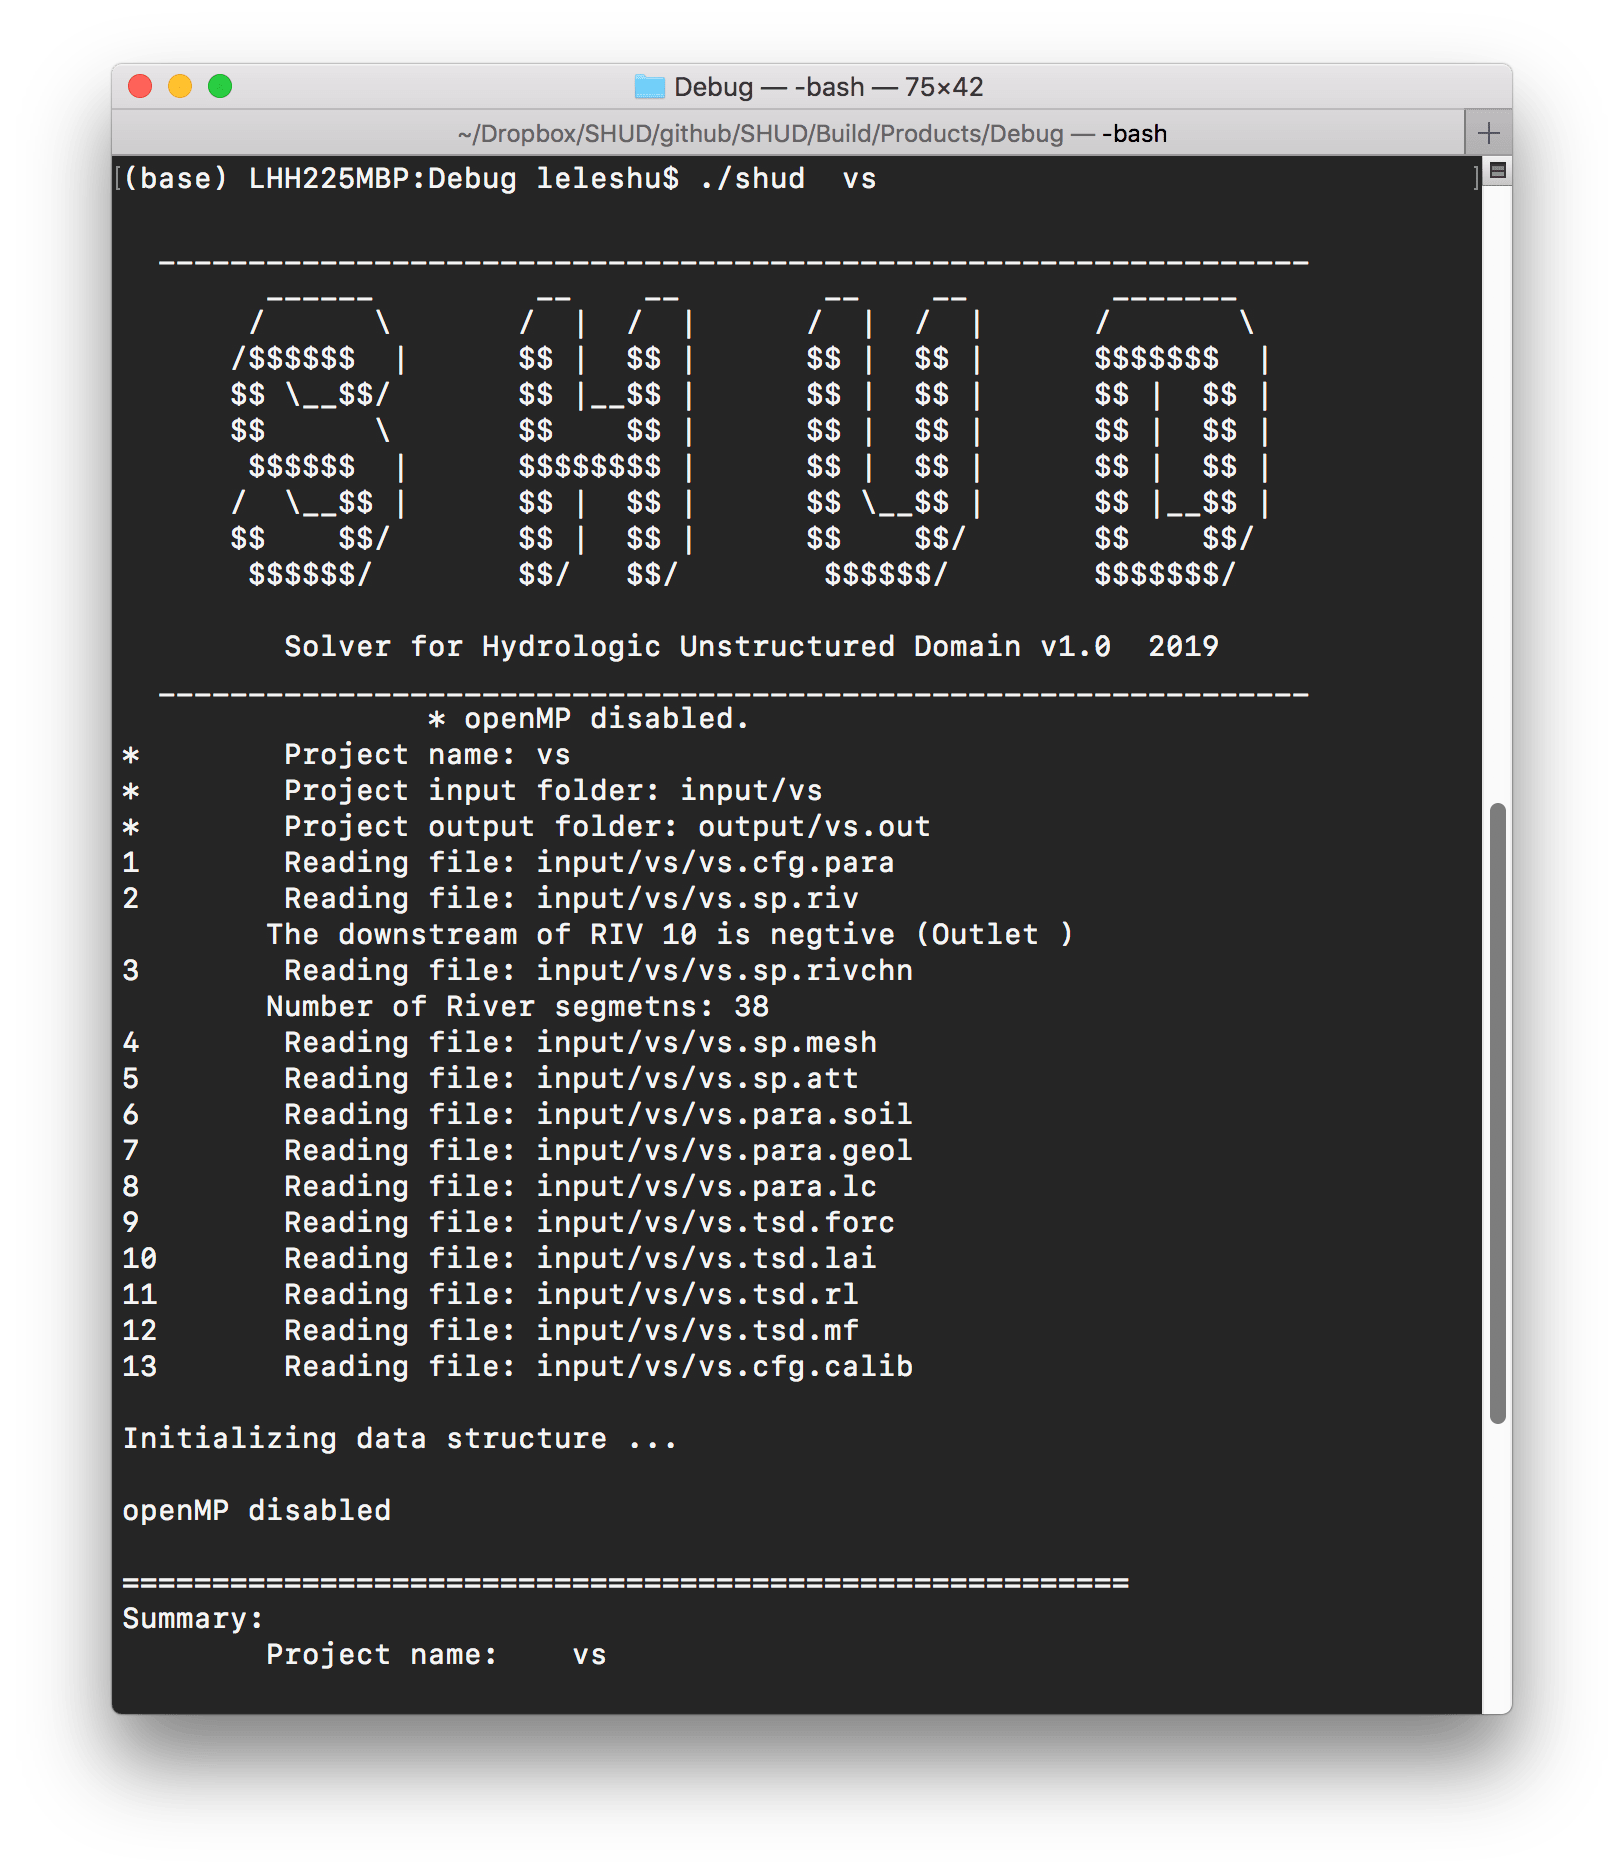
\includegraphics{Fig/CLI_vs.png}

\section{SHUD-tools}\label{shud-tools}

This SHUD-tools is an R package. What you need is to install the package
as a source code package. For example:

\begin{verbatim}
install_github('SHUD-System/shud-tools')
\end{verbatim}

That is all you need to deploy the SHUD-tools.

\chapter{Input files}\label{input-files}

List of input files:

\begin{longtable}[]{@{}ccccc@{}}
\toprule
File & Category & Comments & Header & \# of column\tabularnewline
\midrule
\endhead
.mesh & sp & Domain \textbf{element} (triangular mesh) & Yes
&\tabularnewline
.att & sp & Attribute table of triangular \textbf{elements} & Yes
&\tabularnewline
.riv & sp & \textbf{Rivers} & Yes &\tabularnewline
.rivchn & sp & Topologic relation b/w \textbf{River} and
\textbf{Element} & Yes &\tabularnewline
.calib & cfg & Calibration on physical parameters & Yes &\tabularnewline
.para & cfg & Parameters of the model configurature & Yes
&\tabularnewline
.ic & cfg & Intial conditions & Yes &\tabularnewline
.geol & para & Physical parameters for \textbf{Geology} layers & Yes
&\tabularnewline
.soil & para & Physical parameters for \textbf{Soil} layers & Yes
&\tabularnewline
.lc & para & Physical parameters for \textbf{Land cover} layers & Yes
&\tabularnewline
.forc & tsd & List of files to the Time-series forcing data & Yes
&\tabularnewline
.csv & tsd & Time-series \textbf{forcing} data & Yes &\tabularnewline
.lai & tsd & Time-series \textbf{LAI} data & Yes &\tabularnewline
.obs & tsd & Time-series observational data for calibration purpose only
& Yes &\tabularnewline
.mf & tsd & Time-series \textbf{Melt Factor} data & Yes &\tabularnewline
.rl & tsd & Time-series \textbf{Roughness Length} data & Yes
&\tabularnewline
gis/domain & Shapefile & Shapefile of .mesh file & x & x\tabularnewline
gis/river & Shapefile & Shapefile of .riv file & x & x\tabularnewline
gis/seg & Shapefile & Shapefile of .rivchn file & x & x\tabularnewline
\bottomrule
\end{longtable}

\begin{figure}
\centering
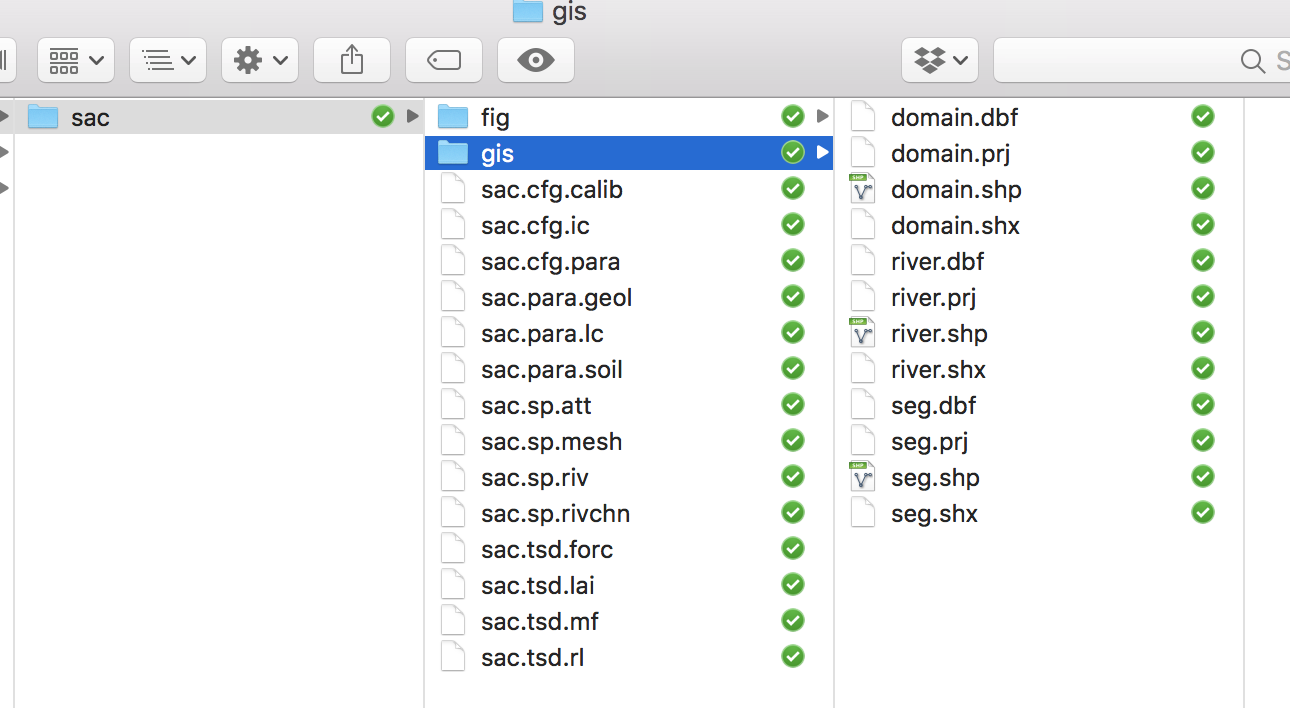
\includegraphics{Fig/IO/Inputfiles.png}
\caption{The screenshot of input files for SHUD}
\end{figure}

The files in folder \emph{gis} and \emph{fig} are not involved in SHUD
modeling, but they are very useful for your data pre- and
post-processing.

\section{Spatial data}\label{spatial-data}

\subsection{.sp.mesh file}\label{sp.mesh-file}

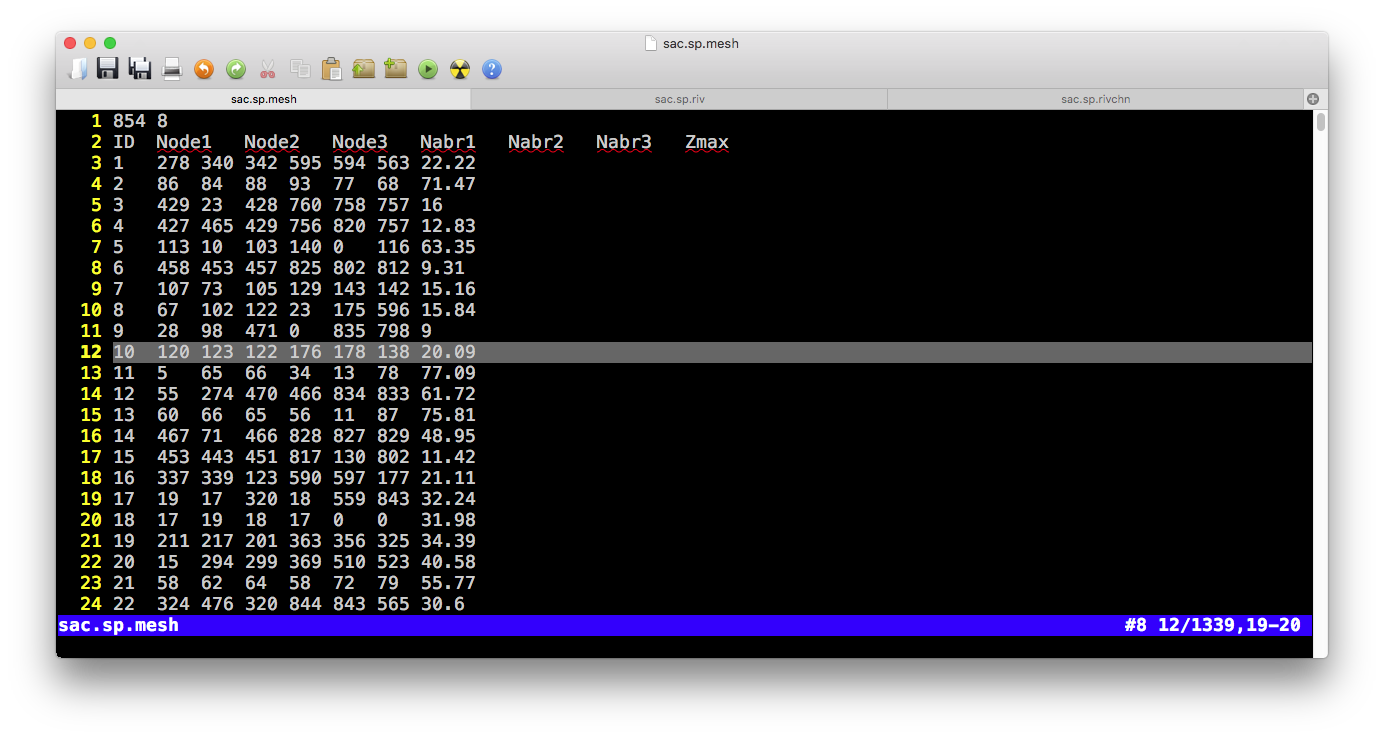
\includegraphics{Fig/IO/sp.mesh1.png}
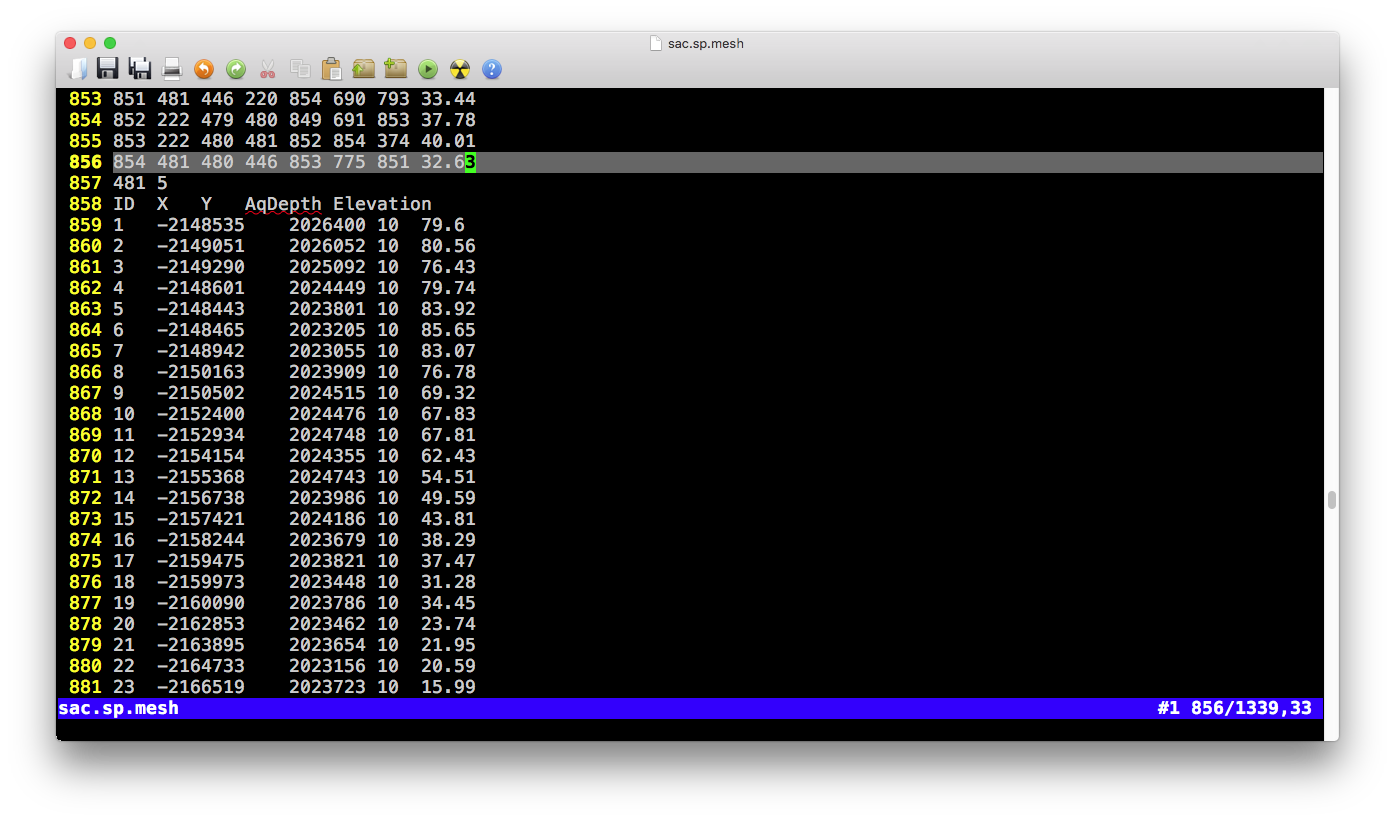
\includegraphics{Fig/IO/sp.mesh2.png} There are two tables in the .mesh
file, the one is a table of elements and the other is a table of nodes
of elements.

\begin{itemize}
\item
  \textbf{Block 1 (Element information)}
\item
  Pre-table
\end{itemize}

\begin{longtable}[]{@{}cc@{}}
\toprule
Value1 & Value2\tabularnewline
\midrule
\endhead
Number of rows ( \(N_{element}\)) & Number of columns
(\(8\))\tabularnewline
\bottomrule
\end{longtable}

\begin{itemize}
\tightlist
\item
  Table
\end{itemize}

\begin{longtable}[]{@{}ccccc@{}}
\toprule
Colname & Meaning & Range & Unit & Comments\tabularnewline
\midrule
\endhead
ID & Index of element \(i\) & 1 \textasciitilde{} \(N_{element}\) & -
&\tabularnewline
Node1 & Node 1 of element \(i\) & 1 \textasciitilde{} \(N_{node}\) & -
&\tabularnewline
Node2 & Node 2 of element \(i\) & 1 \textasciitilde{} \(N_{node}\) & -
&\tabularnewline
Node3 & Node 3 of element \(i\) & 1 \textasciitilde{} \(N_{node}\) & -
&\tabularnewline
Nabr1 & Index of Neighbor 1 of element \(i\) & 1 \textasciitilde{}
\(N_{element}\) & - &\tabularnewline
Nabr2 & Index of Neighbor 2 of element \(i\) & 1 \textasciitilde{}
\(N_{element}\) & - &\tabularnewline
Nabr3 & Index of Neighbor 3 of element \(i\) & 1 \textasciitilde{}
\(N_{element}\) & - &\tabularnewline
Zmax & Surface elevation of element \(i\) & -9999 \textasciitilde{} +inf
& \(m\) &\tabularnewline
\bottomrule
\end{longtable}

\begin{itemize}
\item
  \textbf{Block 2 (node information)}
\item
  Pre-table:
\end{itemize}

\begin{longtable}[]{@{}cc@{}}
\toprule
Value1 & Value2\tabularnewline
\midrule
\endhead
Number of rows ( \(N_{node}\)) & Number of columns
(\(5\))\tabularnewline
\bottomrule
\end{longtable}

\begin{itemize}
\tightlist
\item
  Table
\end{itemize}

\begin{longtable}[]{@{}ccccc@{}}
\toprule
Colname & Meaning & Range & Unit & Comments\tabularnewline
\midrule
\endhead
ID & Index of node \(i\) & 1 \textasciitilde{} \(N_{element}\) & -
&\tabularnewline
X & X coordinate of node \(i\) & 1 \textasciitilde{} \(N_{node}\) & -
&\tabularnewline
Y & Y coordinate of node \(i\) & 1 \textasciitilde{} \(N_{node}\) & -
&\tabularnewline
AqDepth & Thickness of aquifer \(i\) & 0 \textasciitilde{} +inf & \(m\)
&\tabularnewline
Elevation & Surface elevation of node \(i\) & -9999 \textasciitilde{}
+inf & \(m\) &\tabularnewline
\bottomrule
\end{longtable}

\subsection{.sp.att file}\label{sp.att-file}

\begin{figure}
\centering
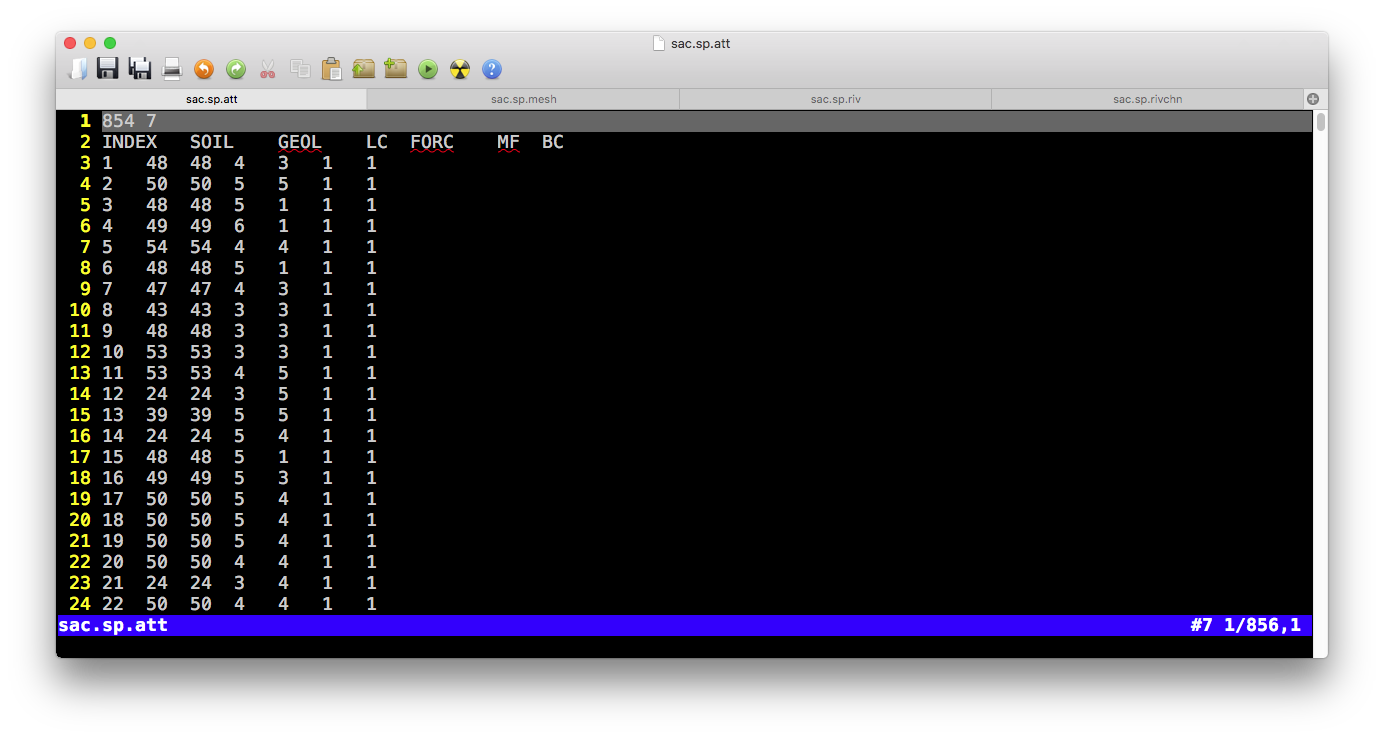
\includegraphics{Fig/IO/sp.att.png}
\caption{Example of .sp.att file}
\end{figure}

\begin{itemize}
\tightlist
\item
  Pre-table
\end{itemize}

\begin{longtable}[]{@{}cc@{}}
\toprule
Value1 & Value2\tabularnewline
\midrule
\endhead
Number of rows ( \(N_{element}\)) & Number of columns
(\(7\))\tabularnewline
\bottomrule
\end{longtable}

\begin{itemize}
\tightlist
\item
  Table
\end{itemize}

\begin{longtable}[]{@{}ccccc@{}}
\toprule
Colname & Meaning & Range & Unit & Comments\tabularnewline
\midrule
\endhead
ID & Index of element \(i\) & 1 \textasciitilde{} \(N_{element}\) & -
&\tabularnewline
SOIL & Index of soil type & 1 \textasciitilde{} \(N_{soil}\) & -
&\tabularnewline
GEOL & Index of geology type & 1 \textasciitilde{} \(N_{geol}\) & -
&\tabularnewline
LC & Index of land cover type & 1 \textasciitilde{} \(N_{lc}\) & - &
\(N_{lc}\) = \(N_{lai}\)\tabularnewline
FORC & Index of forcing site & 1 \textasciitilde{} \(N_{forc}\) & -
&\tabularnewline
MF & Index of melt factor & 1 \textasciitilde{} \(N_{mf}\) & -
&\tabularnewline
BC & Index of boundary condition & 1 \textasciitilde{} \(N_{bc}\) & -
&\tabularnewline
\bottomrule
\end{longtable}

\subsection{.sp.riv file}\label{sp.riv-file}

\begin{figure}
\centering
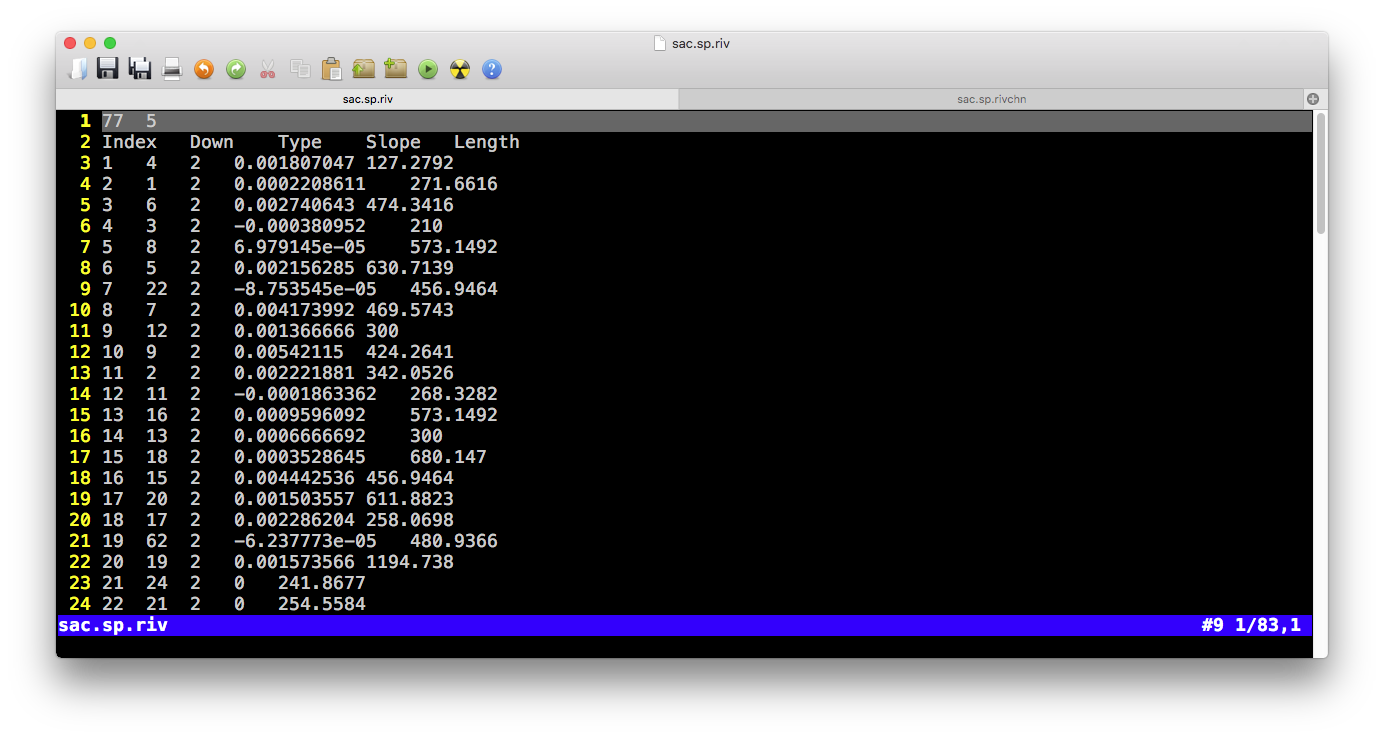
\includegraphics{Fig/IO/sp.riv.png}
\caption{Example of .sp.riv file}
\end{figure}

\begin{itemize}
\tightlist
\item
  Pre-table
\end{itemize}

\begin{longtable}[]{@{}cc@{}}
\toprule
Value1 & Value2\tabularnewline
\midrule
\endhead
Number of rows ( \(N_{riv}\)) & Number of columns (\(5\))\tabularnewline
\bottomrule
\end{longtable}

\begin{itemize}
\tightlist
\item
  Table
\end{itemize}

\begin{longtable}[]{@{}ccccc@{}}
\toprule
\begin{minipage}[b]{0.11\columnwidth}\centering\strut
Colname\strut
\end{minipage} & \begin{minipage}[b]{0.25\columnwidth}\centering\strut
Meaning\strut
\end{minipage} & \begin{minipage}[b]{0.11\columnwidth}\centering\strut
Range\strut
\end{minipage} & \begin{minipage}[b]{0.11\columnwidth}\centering\strut
Unit\strut
\end{minipage} & \begin{minipage}[b]{0.29\columnwidth}\centering\strut
Comments\strut
\end{minipage}\tabularnewline
\midrule
\endhead
\begin{minipage}[t]{0.11\columnwidth}\centering\strut
ID\strut
\end{minipage} & \begin{minipage}[t]{0.25\columnwidth}\centering\strut
Index of river \(i\)\strut
\end{minipage} & \begin{minipage}[t]{0.11\columnwidth}\centering\strut
1 \textasciitilde{} \(N_{river}\)\strut
\end{minipage} & \begin{minipage}[t]{0.11\columnwidth}\centering\strut
-\strut
\end{minipage} & \begin{minipage}[t]{0.29\columnwidth}\centering\strut
\strut
\end{minipage}\tabularnewline
\begin{minipage}[t]{0.11\columnwidth}\centering\strut
DOWN\strut
\end{minipage} & \begin{minipage}[t]{0.25\columnwidth}\centering\strut
Index of downstream river\strut
\end{minipage} & \begin{minipage}[t]{0.11\columnwidth}\centering\strut
1 \textasciitilde{} \(N_{river}\)\strut
\end{minipage} & \begin{minipage}[t]{0.11\columnwidth}\centering\strut
-\strut
\end{minipage} & \begin{minipage}[t]{0.29\columnwidth}\centering\strut
Negative vlaue indicates outlet\strut
\end{minipage}\tabularnewline
\begin{minipage}[t]{0.11\columnwidth}\centering\strut
Type\strut
\end{minipage} & \begin{minipage}[t]{0.25\columnwidth}\centering\strut
Index of river parameters\strut
\end{minipage} & \begin{minipage}[t]{0.11\columnwidth}\centering\strut
1 \textasciitilde{} \(N_{rivertype}\)\strut
\end{minipage} & \begin{minipage}[t]{0.11\columnwidth}\centering\strut
-\strut
\end{minipage} & \begin{minipage}[t]{0.29\columnwidth}\centering\strut
\strut
\end{minipage}\tabularnewline
\begin{minipage}[t]{0.11\columnwidth}\centering\strut
Slope\strut
\end{minipage} & \begin{minipage}[t]{0.25\columnwidth}\centering\strut
Slope of river bed\strut
\end{minipage} & \begin{minipage}[t]{0.11\columnwidth}\centering\strut
-10 \textasciitilde{} 10\strut
\end{minipage} & \begin{minipage}[t]{0.11\columnwidth}\centering\strut
\(m/m\)\strut
\end{minipage} & \begin{minipage}[t]{0.29\columnwidth}\centering\strut
Height/Length\strut
\end{minipage}\tabularnewline
\begin{minipage}[t]{0.11\columnwidth}\centering\strut
Length\strut
\end{minipage} & \begin{minipage}[t]{0.25\columnwidth}\centering\strut
Length of the river \(i\)\strut
\end{minipage} & \begin{minipage}[t]{0.11\columnwidth}\centering\strut
0 \textasciitilde{} inf\strut
\end{minipage} & \begin{minipage}[t]{0.11\columnwidth}\centering\strut
\(m\)\strut
\end{minipage} & \begin{minipage}[t]{0.29\columnwidth}\centering\strut
\strut
\end{minipage}\tabularnewline
\bottomrule
\end{longtable}

\subsection{.sp.rivseg file}\label{sp.rivseg-file}

\begin{figure}
\centering
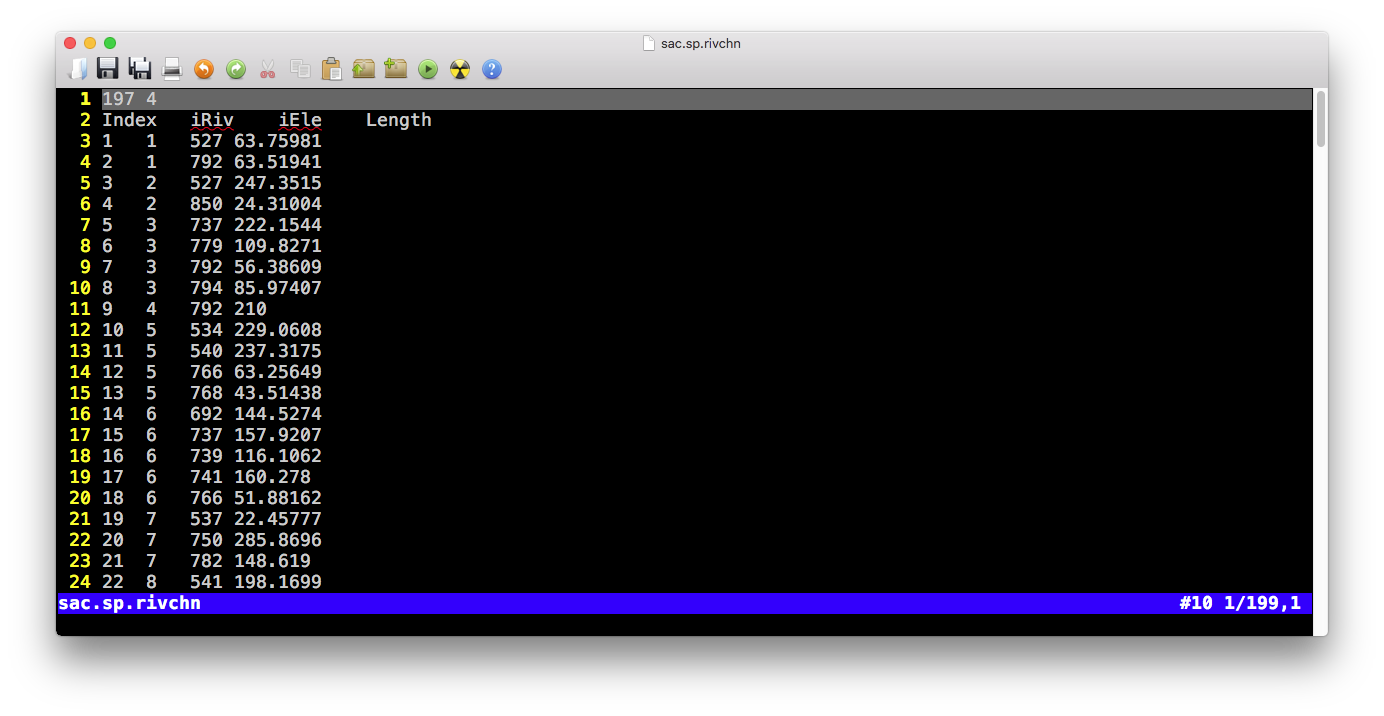
\includegraphics{Fig/IO/sp.rivchn.png}
\caption{Example of .sp.rivseg file}
\end{figure}

\begin{itemize}
\tightlist
\item
  Pre-table
\end{itemize}

\begin{longtable}[]{@{}cc@{}}
\toprule
Value1 & Value2\tabularnewline
\midrule
\endhead
Number of rows ( \(N_{segment}\)) & Number of columns
(\(4\))\tabularnewline
\bottomrule
\end{longtable}

\begin{itemize}
\tightlist
\item
  Table
\end{itemize}

\begin{longtable}[]{@{}ccccc@{}}
\toprule
Colname & Meaning & Range & Unit & Comments\tabularnewline
\midrule
\endhead
ID & Index of segments \(i\) & 1 \textasciitilde{} \(N_{segment}\) & -
&\tabularnewline
iRiv & Index of river & 1 \textasciitilde{} \(N_{river}\) & -
&\tabularnewline
iEle & Index of element & 1 \textasciitilde{} \(N_{element}\) & -
&\tabularnewline
Length & Length of the segments \(i\) & 0 \textasciitilde{} inf & \(m\)
&\tabularnewline
\bottomrule
\end{longtable}

\section{Model configuration files}\label{model-configuration-files}

\subsection{.cfg.para file}\label{cfg.para-file}

\begin{figure}
\centering
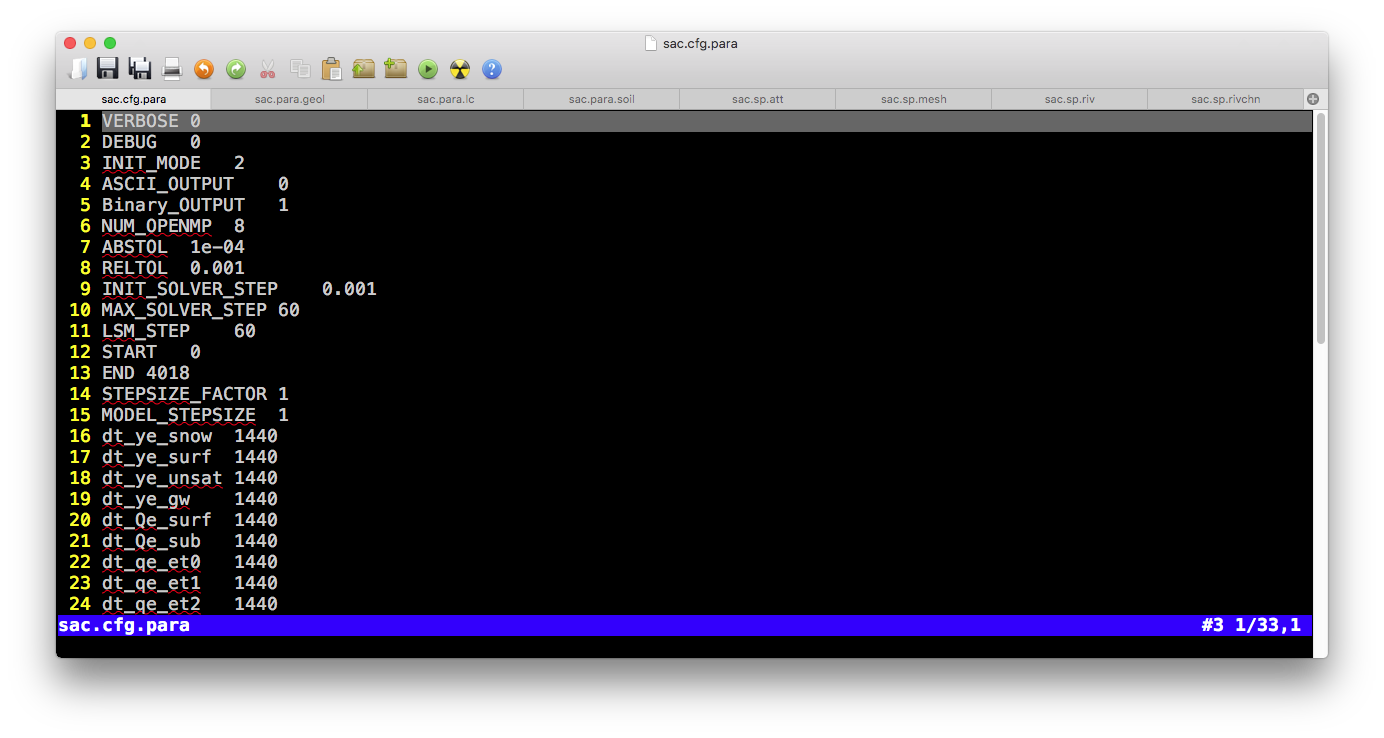
\includegraphics{Fig/IO/cfg.para.png}
\caption{Example of .cfg.para file}
\end{figure}

\begin{itemize}
\tightlist
\item
  Table
\end{itemize}

\begin{longtable}[]{@{}ccccc@{}}
\toprule
\begin{minipage}[b]{0.17\columnwidth}\centering\strut
Colname\strut
\end{minipage} & \begin{minipage}[b]{0.23\columnwidth}\centering\strut
Meaning\strut
\end{minipage} & \begin{minipage}[b]{0.10\columnwidth}\centering\strut
Range\strut
\end{minipage} & \begin{minipage}[b]{0.10\columnwidth}\centering\strut
Unit\strut
\end{minipage} & \begin{minipage}[b]{0.26\columnwidth}\centering\strut
Comments\strut
\end{minipage}\tabularnewline
\midrule
\endhead
\begin{minipage}[t]{0.17\columnwidth}\centering\strut
VERBOSE\strut
\end{minipage} & \begin{minipage}[t]{0.23\columnwidth}\centering\strut
Verbose mode\strut
\end{minipage} & \begin{minipage}[t]{0.10\columnwidth}\centering\strut
-\strut
\end{minipage} & \begin{minipage}[t]{0.10\columnwidth}\centering\strut
-\strut
\end{minipage} & \begin{minipage}[t]{0.26\columnwidth}\centering\strut
\strut
\end{minipage}\tabularnewline
\begin{minipage}[t]{0.17\columnwidth}\centering\strut
DEBUG\strut
\end{minipage} & \begin{minipage}[t]{0.23\columnwidth}\centering\strut
Debug mode\strut
\end{minipage} & \begin{minipage}[t]{0.10\columnwidth}\centering\strut
-\strut
\end{minipage} & \begin{minipage}[t]{0.10\columnwidth}\centering\strut
-\strut
\end{minipage} & \begin{minipage}[t]{0.26\columnwidth}\centering\strut
\strut
\end{minipage}\tabularnewline
\begin{minipage}[t]{0.17\columnwidth}\centering\strut
INIT\_MODE\strut
\end{minipage} & \begin{minipage}[t]{0.23\columnwidth}\centering\strut
Initial condition mode\strut
\end{minipage} & \begin{minipage}[t]{0.10\columnwidth}\centering\strut
1,2,3\strut
\end{minipage} & \begin{minipage}[t]{0.10\columnwidth}\centering\strut
-\strut
\end{minipage} & \begin{minipage}[t]{0.26\columnwidth}\centering\strut
1=Dry condition, 2=Relief conditon, 3=Warm start\strut
\end{minipage}\tabularnewline
\begin{minipage}[t]{0.17\columnwidth}\centering\strut
ASCII\_OUTPUT\strut
\end{minipage} & \begin{minipage}[t]{0.23\columnwidth}\centering\strut
ASCII ouput\strut
\end{minipage} & \begin{minipage}[t]{0.10\columnwidth}\centering\strut
1/0\strut
\end{minipage} & \begin{minipage}[t]{0.10\columnwidth}\centering\strut
-\strut
\end{minipage} & \begin{minipage}[t]{0.26\columnwidth}\centering\strut
\strut
\end{minipage}\tabularnewline
\begin{minipage}[t]{0.17\columnwidth}\centering\strut
Binary\_OUTPUT\strut
\end{minipage} & \begin{minipage}[t]{0.23\columnwidth}\centering\strut
Binary output\strut
\end{minipage} & \begin{minipage}[t]{0.10\columnwidth}\centering\strut
1/0\strut
\end{minipage} & \begin{minipage}[t]{0.10\columnwidth}\centering\strut
-\strut
\end{minipage} & \begin{minipage}[t]{0.26\columnwidth}\centering\strut
\strut
\end{minipage}\tabularnewline
\begin{minipage}[t]{0.17\columnwidth}\centering\strut
NUM\_OPENMP\strut
\end{minipage} & \begin{minipage}[t]{0.23\columnwidth}\centering\strut
Number of threads for OpenMP\strut
\end{minipage} & \begin{minipage}[t]{0.10\columnwidth}\centering\strut
0 \textasciitilde{} \(N_{threads}\)\strut
\end{minipage} & \begin{minipage}[t]{0.10\columnwidth}\centering\strut
-\strut
\end{minipage} & \begin{minipage}[t]{0.26\columnwidth}\centering\strut
\strut
\end{minipage}\tabularnewline
\begin{minipage}[t]{0.17\columnwidth}\centering\strut
ABSTOL\strut
\end{minipage} & \begin{minipage}[t]{0.23\columnwidth}\centering\strut
Abosolute tolerance for CVODE solver\strut
\end{minipage} & \begin{minipage}[t]{0.10\columnwidth}\centering\strut
1e-6 \textasciitilde{} 0.1\strut
\end{minipage} & \begin{minipage}[t]{0.10\columnwidth}\centering\strut
-\strut
\end{minipage} & \begin{minipage}[t]{0.26\columnwidth}\centering\strut
\strut
\end{minipage}\tabularnewline
\begin{minipage}[t]{0.17\columnwidth}\centering\strut
RELTOL\strut
\end{minipage} & \begin{minipage}[t]{0.23\columnwidth}\centering\strut
Relative tolerance for CVODE solver\strut
\end{minipage} & \begin{minipage}[t]{0.10\columnwidth}\centering\strut
1e-6 \textasciitilde{} 0.1\strut
\end{minipage} & \begin{minipage}[t]{0.10\columnwidth}\centering\strut
-\strut
\end{minipage} & \begin{minipage}[t]{0.26\columnwidth}\centering\strut
\strut
\end{minipage}\tabularnewline
\begin{minipage}[t]{0.17\columnwidth}\centering\strut
INIT\_SOLVER\_STEP\strut
\end{minipage} & \begin{minipage}[t]{0.23\columnwidth}\centering\strut
Initial time step for CVODE solver\strut
\end{minipage} & \begin{minipage}[t]{0.10\columnwidth}\centering\strut
?\strut
\end{minipage} & \begin{minipage}[t]{0.10\columnwidth}\centering\strut
-\strut
\end{minipage} & \begin{minipage}[t]{0.26\columnwidth}\centering\strut
\strut
\end{minipage}\tabularnewline
\begin{minipage}[t]{0.17\columnwidth}\centering\strut
MAX\_SOLVER\_STEP\strut
\end{minipage} & \begin{minipage}[t]{0.23\columnwidth}\centering\strut
Maximum time step for CVODE solver\strut
\end{minipage} & \begin{minipage}[t]{0.10\columnwidth}\centering\strut
?\strut
\end{minipage} & \begin{minipage}[t]{0.10\columnwidth}\centering\strut
-\strut
\end{minipage} & \begin{minipage}[t]{0.26\columnwidth}\centering\strut
\strut
\end{minipage}\tabularnewline
\begin{minipage}[t]{0.17\columnwidth}\centering\strut
ET\_STEP\strut
\end{minipage} & \begin{minipage}[t]{0.23\columnwidth}\centering\strut
Time step of Evapotranspiration\strut
\end{minipage} & \begin{minipage}[t]{0.10\columnwidth}\centering\strut
1\textasciitilde{}360\strut
\end{minipage} & \begin{minipage}[t]{0.10\columnwidth}\centering\strut
\(min\)\strut
\end{minipage} & \begin{minipage}[t]{0.26\columnwidth}\centering\strut
\strut
\end{minipage}\tabularnewline
\begin{minipage}[t]{0.17\columnwidth}\centering\strut
START\strut
\end{minipage} & \begin{minipage}[t]{0.23\columnwidth}\centering\strut
Start Time\strut
\end{minipage} & \begin{minipage}[t]{0.10\columnwidth}\centering\strut
0 \textasciitilde{} inf\strut
\end{minipage} & \begin{minipage}[t]{0.10\columnwidth}\centering\strut
\(day\)\strut
\end{minipage} & \begin{minipage}[t]{0.26\columnwidth}\centering\strut
\strut
\end{minipage}\tabularnewline
\begin{minipage}[t]{0.17\columnwidth}\centering\strut
END\strut
\end{minipage} & \begin{minipage}[t]{0.23\columnwidth}\centering\strut
End Time\strut
\end{minipage} & \begin{minipage}[t]{0.10\columnwidth}\centering\strut
-\strut
\end{minipage} & \begin{minipage}[t]{0.10\columnwidth}\centering\strut
\(day\)\strut
\end{minipage} & \begin{minipage}[t]{0.26\columnwidth}\centering\strut
\strut
\end{minipage}\tabularnewline
\begin{minipage}[t]{0.17\columnwidth}\centering\strut
dt\_ye\_snow\strut
\end{minipage} & \begin{minipage}[t]{0.23\columnwidth}\centering\strut
Time step of output snow storage\strut
\end{minipage} & \begin{minipage}[t]{0.10\columnwidth}\centering\strut
0 \textasciitilde{} inf\strut
\end{minipage} & \begin{minipage}[t]{0.10\columnwidth}\centering\strut
\(min\)\strut
\end{minipage} & \begin{minipage}[t]{0.26\columnwidth}\centering\strut
\strut
\end{minipage}\tabularnewline
\begin{minipage}[t]{0.17\columnwidth}\centering\strut
dt\_ye\_surf\strut
\end{minipage} & \begin{minipage}[t]{0.23\columnwidth}\centering\strut
Time step of output surface storage\strut
\end{minipage} & \begin{minipage}[t]{0.10\columnwidth}\centering\strut
0 \textasciitilde{} inf\strut
\end{minipage} & \begin{minipage}[t]{0.10\columnwidth}\centering\strut
\(min\)\strut
\end{minipage} & \begin{minipage}[t]{0.26\columnwidth}\centering\strut
\strut
\end{minipage}\tabularnewline
\begin{minipage}[t]{0.17\columnwidth}\centering\strut
dt\_ye\_unsat\strut
\end{minipage} & \begin{minipage}[t]{0.23\columnwidth}\centering\strut
Time step of output unsaturated storage\strut
\end{minipage} & \begin{minipage}[t]{0.10\columnwidth}\centering\strut
0 \textasciitilde{} inf\strut
\end{minipage} & \begin{minipage}[t]{0.10\columnwidth}\centering\strut
\(min\)\strut
\end{minipage} & \begin{minipage}[t]{0.26\columnwidth}\centering\strut
\strut
\end{minipage}\tabularnewline
\begin{minipage}[t]{0.17\columnwidth}\centering\strut
dt\_ye\_gw\strut
\end{minipage} & \begin{minipage}[t]{0.23\columnwidth}\centering\strut
Time step of output groundwater head\strut
\end{minipage} & \begin{minipage}[t]{0.10\columnwidth}\centering\strut
0 \textasciitilde{} inf\strut
\end{minipage} & \begin{minipage}[t]{0.10\columnwidth}\centering\strut
\(min\)\strut
\end{minipage} & \begin{minipage}[t]{0.26\columnwidth}\centering\strut
\strut
\end{minipage}\tabularnewline
\begin{minipage}[t]{0.17\columnwidth}\centering\strut
dt\_Qe\_surf\strut
\end{minipage} & \begin{minipage}[t]{0.23\columnwidth}\centering\strut
Time step of output surface element flux\strut
\end{minipage} & \begin{minipage}[t]{0.10\columnwidth}\centering\strut
0 \textasciitilde{} inf\strut
\end{minipage} & \begin{minipage}[t]{0.10\columnwidth}\centering\strut
\(min\)\strut
\end{minipage} & \begin{minipage}[t]{0.26\columnwidth}\centering\strut
\strut
\end{minipage}\tabularnewline
\begin{minipage}[t]{0.17\columnwidth}\centering\strut
dt\_Qe\_sub\strut
\end{minipage} & \begin{minipage}[t]{0.23\columnwidth}\centering\strut
Time step of output subsurface element flux\strut
\end{minipage} & \begin{minipage}[t]{0.10\columnwidth}\centering\strut
0 \textasciitilde{} inf\strut
\end{minipage} & \begin{minipage}[t]{0.10\columnwidth}\centering\strut
\(min\)\strut
\end{minipage} & \begin{minipage}[t]{0.26\columnwidth}\centering\strut
\strut
\end{minipage}\tabularnewline
\begin{minipage}[t]{0.17\columnwidth}\centering\strut
dt\_qe\_et0\strut
\end{minipage} & \begin{minipage}[t]{0.23\columnwidth}\centering\strut
Time step of output element flux, interception\strut
\end{minipage} & \begin{minipage}[t]{0.10\columnwidth}\centering\strut
0 \textasciitilde{} inf\strut
\end{minipage} & \begin{minipage}[t]{0.10\columnwidth}\centering\strut
\(min\)\strut
\end{minipage} & \begin{minipage}[t]{0.26\columnwidth}\centering\strut
\strut
\end{minipage}\tabularnewline
\begin{minipage}[t]{0.17\columnwidth}\centering\strut
dt\_qe\_et1\strut
\end{minipage} & \begin{minipage}[t]{0.23\columnwidth}\centering\strut
Time step of output element flux, transpiration\strut
\end{minipage} & \begin{minipage}[t]{0.10\columnwidth}\centering\strut
0 \textasciitilde{} inf\strut
\end{minipage} & \begin{minipage}[t]{0.10\columnwidth}\centering\strut
\(min\)\strut
\end{minipage} & \begin{minipage}[t]{0.26\columnwidth}\centering\strut
\strut
\end{minipage}\tabularnewline
\begin{minipage}[t]{0.17\columnwidth}\centering\strut
dt\_qe\_et2\strut
\end{minipage} & \begin{minipage}[t]{0.23\columnwidth}\centering\strut
Time step of output element flux, evaporation\strut
\end{minipage} & \begin{minipage}[t]{0.10\columnwidth}\centering\strut
0 \textasciitilde{} inf\strut
\end{minipage} & \begin{minipage}[t]{0.10\columnwidth}\centering\strut
\(min\)\strut
\end{minipage} & \begin{minipage}[t]{0.26\columnwidth}\centering\strut
\strut
\end{minipage}\tabularnewline
\begin{minipage}[t]{0.17\columnwidth}\centering\strut
dt\_qe\_etp\strut
\end{minipage} & \begin{minipage}[t]{0.23\columnwidth}\centering\strut
Time step of output element flux, potential ET\strut
\end{minipage} & \begin{minipage}[t]{0.10\columnwidth}\centering\strut
0 \textasciitilde{} inf\strut
\end{minipage} & \begin{minipage}[t]{0.10\columnwidth}\centering\strut
\(min\)\strut
\end{minipage} & \begin{minipage}[t]{0.26\columnwidth}\centering\strut
\strut
\end{minipage}\tabularnewline
\begin{minipage}[t]{0.17\columnwidth}\centering\strut
dt\_qe\_prcp\strut
\end{minipage} & \begin{minipage}[t]{0.23\columnwidth}\centering\strut
Time step of output element flux, interception\strut
\end{minipage} & \begin{minipage}[t]{0.10\columnwidth}\centering\strut
0 \textasciitilde{} inf\strut
\end{minipage} & \begin{minipage}[t]{0.10\columnwidth}\centering\strut
\(min\)\strut
\end{minipage} & \begin{minipage}[t]{0.26\columnwidth}\centering\strut
\strut
\end{minipage}\tabularnewline
\begin{minipage}[t]{0.17\columnwidth}\centering\strut
dt\_qe\_infil\strut
\end{minipage} & \begin{minipage}[t]{0.23\columnwidth}\centering\strut
Time step of output element flux, interception\strut
\end{minipage} & \begin{minipage}[t]{0.10\columnwidth}\centering\strut
0 \textasciitilde{} inf\strut
\end{minipage} & \begin{minipage}[t]{0.10\columnwidth}\centering\strut
\(min\)\strut
\end{minipage} & \begin{minipage}[t]{0.26\columnwidth}\centering\strut
\strut
\end{minipage}\tabularnewline
\begin{minipage}[t]{0.17\columnwidth}\centering\strut
dt\_qe\_rech\strut
\end{minipage} & \begin{minipage}[t]{0.23\columnwidth}\centering\strut
Time step of output element flux, interception\strut
\end{minipage} & \begin{minipage}[t]{0.10\columnwidth}\centering\strut
0 \textasciitilde{} inf\strut
\end{minipage} & \begin{minipage}[t]{0.10\columnwidth}\centering\strut
\(min\)\strut
\end{minipage} & \begin{minipage}[t]{0.26\columnwidth}\centering\strut
\strut
\end{minipage}\tabularnewline
\begin{minipage}[t]{0.17\columnwidth}\centering\strut
dt\_yr\_stage\strut
\end{minipage} & \begin{minipage}[t]{0.23\columnwidth}\centering\strut
Time step of output river stage\strut
\end{minipage} & \begin{minipage}[t]{0.10\columnwidth}\centering\strut
0 \textasciitilde{} inf\strut
\end{minipage} & \begin{minipage}[t]{0.10\columnwidth}\centering\strut
\(min\)\strut
\end{minipage} & \begin{minipage}[t]{0.26\columnwidth}\centering\strut
\strut
\end{minipage}\tabularnewline
\begin{minipage}[t]{0.17\columnwidth}\centering\strut
dt\_Qr\_down\strut
\end{minipage} & \begin{minipage}[t]{0.23\columnwidth}\centering\strut
Time step of output river flux, downstream\strut
\end{minipage} & \begin{minipage}[t]{0.10\columnwidth}\centering\strut
0 \textasciitilde{} inf\strut
\end{minipage} & \begin{minipage}[t]{0.10\columnwidth}\centering\strut
\(min\)\strut
\end{minipage} & \begin{minipage}[t]{0.26\columnwidth}\centering\strut
\strut
\end{minipage}\tabularnewline
\begin{minipage}[t]{0.17\columnwidth}\centering\strut
dt\_Qr\_surf\strut
\end{minipage} & \begin{minipage}[t]{0.23\columnwidth}\centering\strut
Time step of output river flux, surface flow\strut
\end{minipage} & \begin{minipage}[t]{0.10\columnwidth}\centering\strut
0 \textasciitilde{} inf\strut
\end{minipage} & \begin{minipage}[t]{0.10\columnwidth}\centering\strut
\(min\)\strut
\end{minipage} & \begin{minipage}[t]{0.26\columnwidth}\centering\strut
\strut
\end{minipage}\tabularnewline
\begin{minipage}[t]{0.17\columnwidth}\centering\strut
dt\_Qr\_sub\strut
\end{minipage} & \begin{minipage}[t]{0.23\columnwidth}\centering\strut
Time step of output river flux, base flow\strut
\end{minipage} & \begin{minipage}[t]{0.10\columnwidth}\centering\strut
0 \textasciitilde{} inf\strut
\end{minipage} & \begin{minipage}[t]{0.10\columnwidth}\centering\strut
\(min\)\strut
\end{minipage} & \begin{minipage}[t]{0.26\columnwidth}\centering\strut
\strut
\end{minipage}\tabularnewline
\begin{minipage}[t]{0.17\columnwidth}\centering\strut
dt\_Qr\_up\strut
\end{minipage} & \begin{minipage}[t]{0.23\columnwidth}\centering\strut
Time step of output river flux, upstream\strut
\end{minipage} & \begin{minipage}[t]{0.10\columnwidth}\centering\strut
0 \textasciitilde{} inf\strut
\end{minipage} & \begin{minipage}[t]{0.10\columnwidth}\centering\strut
\(min\)\strut
\end{minipage} & \begin{minipage}[t]{0.26\columnwidth}\centering\strut
\strut
\end{minipage}\tabularnewline
\bottomrule
\end{longtable}

\subsection{.cfg.calib file}\label{cfg.calib-file}

\begin{figure}
\centering
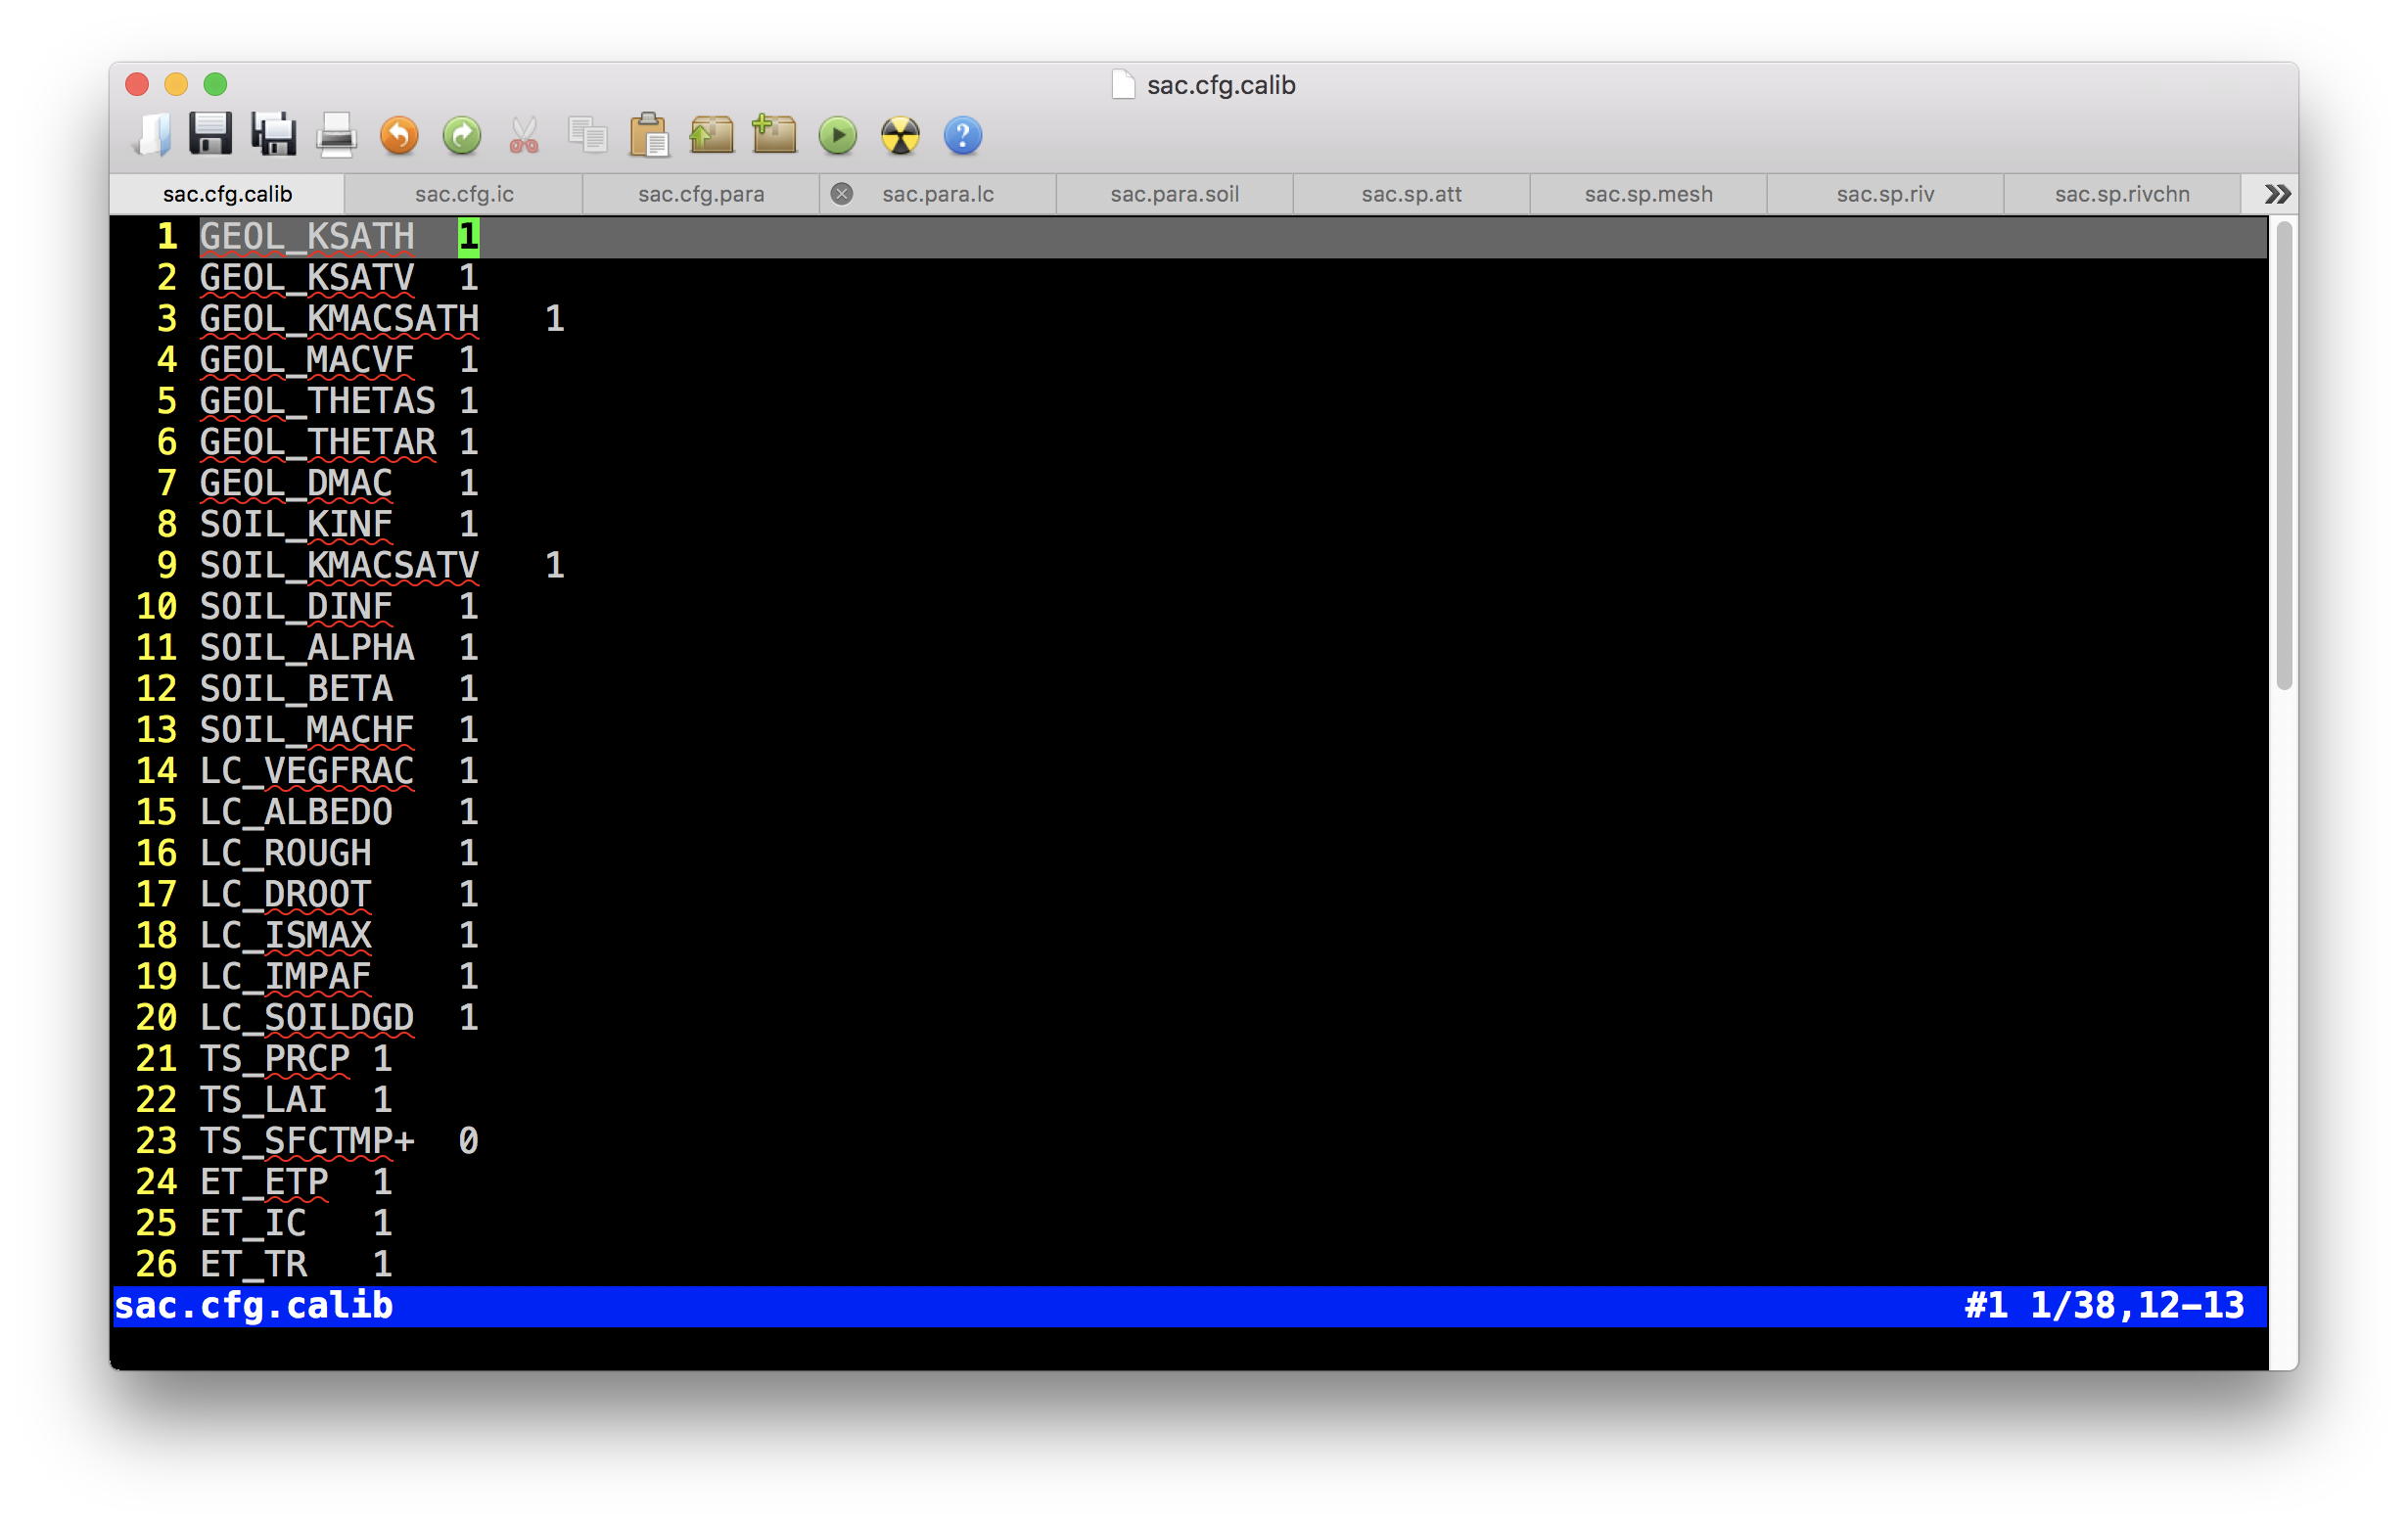
\includegraphics{Fig/IO/cfg.calib.png}
\caption{Example of .cfg.calib file}
\end{figure}

\begin{itemize}
\tightlist
\item
  Table
\end{itemize}

\begin{longtable}[]{@{}ccccc@{}}
\toprule
Colname & Meaning & Range & Unit & Comments\tabularnewline
\midrule
\endhead
GEOL\_KSATH & Horizontal conductivity of ground water & ? & -
&\tabularnewline
GEOL\_KSATV & Vertical conductivity of ground water & ? & -
&\tabularnewline
GEOL\_KMACSATH & Horizontal conductivity of macropore & ? & -
&\tabularnewline
GEOL\_DMAC & Macropore depth & & - &\tabularnewline
GEOL\_THETAS & Porosity, saturated soil moisture & & - &\tabularnewline
GEOL\_THETAR & Residual soil moisture & & - &\tabularnewline
GEOL\_MACVF & Vertical macropore areal fraction & & - &\tabularnewline
SOIL\_KINF & Vertical conductivity of top soil & ? & - &\tabularnewline
SOIL\_KMACSATV & Vertical conductivity of soil macropore & ? & -
&\tabularnewline
SOIL\_DINF & Infiltration depth & ? & - &\tabularnewline
SOIL\_DROOT & Root depth & & - &\tabularnewline
SOIL\_ALPHA & \(\alpha\) value in van Genuchten equation & & -
&\tabularnewline
SOIL\_BETA & \(\beta\) value in van Genuchten equation & & -
&\tabularnewline
SOIL\_MACHF & Horizontal macropore areal fraction & & - &\tabularnewline
LC\_VEGFRAC & Vegetation fraction & & - &\tabularnewline
LC\_ALBEDO & Emissitive reflection ratio & & - &\tabularnewline
LC\_ROUGH & Manning's roughness of element surface & & -
&\tabularnewline
LC\_SOILDGD & Soil degradation & & - &\tabularnewline
LC\_IMPAF & Impervious areal fraction & & - &\tabularnewline
LC\_ISMAX & Maximum interception & & - &\tabularnewline
AQ\_DEPTH+ & Thichness of aquifer & & \(m\) &\tabularnewline
TS\_PRCP & Precipitation & & - &\tabularnewline
TS\_SFCTMP+ & Temperature & & \(C\) &\tabularnewline
ET\_ETP & Transpiration & & - &\tabularnewline
ET\_IC & Interception & & - &\tabularnewline
ET\_TR & Evaporation & & - &\tabularnewline
ET\_SOIL & Evaporation & & - &\tabularnewline
RIV\_ROUGH & Manning's roughness of river & & - &\tabularnewline
RIV\_KH & Conductivity of river bed & & - &\tabularnewline
RIV\_DPTH+ & Depth of river cross section & & \(m\) &\tabularnewline
RIV\_WDTH+ & Width of river cross section & & \(m\) &\tabularnewline
RIV\_SINU & Sinuosity of river path & & - &\tabularnewline
RIV\_CWR & \(C_{wr}\) in Chezy equation & & - &\tabularnewline
RIV\_BSLOPE+ & Slope of river bed & & \(m/m\) &\tabularnewline
IC\_GW+ & Initial condition of groundwater & & \(m\) &\tabularnewline
IC\_RIV+ & Initial condition of river stage & & \(m\) &\tabularnewline
\bottomrule
\end{longtable}

\subsection{.cfg.ic file}\label{cfg.ic-file}

\begin{figure}
\centering
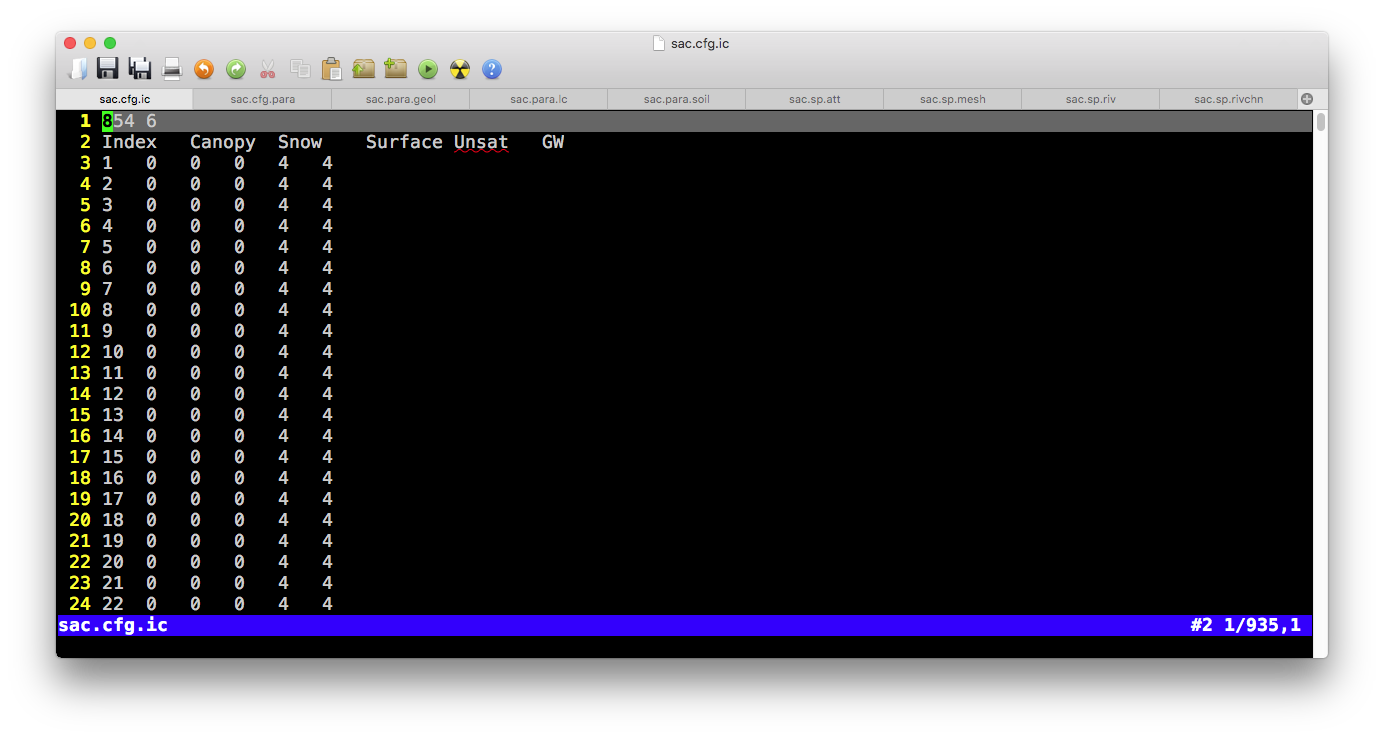
\includegraphics{Fig/IO/cfg.ic.png}
\caption{Example of .cfg.ic file}
\end{figure}

\begin{itemize}
\item
  \textbf{Block 1 (Element initial condition)}
\item
  Pre-table
\end{itemize}

\begin{longtable}[]{@{}cc@{}}
\toprule
Value1 & Value2\tabularnewline
\midrule
\endhead
Number of rows ( \(N_{element}\)) & Number of columns
(\(6\))\tabularnewline
\bottomrule
\end{longtable}

\begin{itemize}
\tightlist
\item
  Table
\end{itemize}

\begin{longtable}[]{@{}ccccc@{}}
\toprule
Colname & Meaning & Range & Unit & Comments\tabularnewline
\midrule
\endhead
ID & Index of element \(i\) & 1 \textasciitilde{} \(N_{element}\) & -
&\tabularnewline
Canopy & Canopy storage of element \(i\) & 0 \textasciitilde{} inf &
\(m\) &\tabularnewline
Snow & Snow storage of element \(i\) & 0 \textasciitilde{} inf & \(m\)
&\tabularnewline
Surface & Surface storage of element \(i\) & 0 \textasciitilde{} inf &
\(m\) &\tabularnewline
Unsat & Unsaturated storage of element \(i\) & 0 \textasciitilde{} inf &
\(m\) &\tabularnewline
GW & Groundwater head of element \(i\) & 0 \textasciitilde{} inf & \(m\)
&\tabularnewline
\bottomrule
\end{longtable}

\begin{itemize}
\item
  \textbf{Block 2 (river initial condition)}
\item
  Pre-table:
\end{itemize}

\begin{longtable}[]{@{}cc@{}}
\toprule
Value1 & Value2\tabularnewline
\midrule
\endhead
Number of rows ( \(N_{riv}\)) & Number of columns (\(2\))\tabularnewline
\bottomrule
\end{longtable}

\begin{itemize}
\tightlist
\item
  Table
\end{itemize}

\begin{longtable}[]{@{}ccccc@{}}
\toprule
Colname & Meaning & Range & Unit & Comments\tabularnewline
\midrule
\endhead
ID & Index of river \(i\) & 1 \textasciitilde{} \(N_{riv}\) & -
&\tabularnewline
Stage & Stage of river \(i\) & 0 \textasciitilde{} inf & \(m\)
&\tabularnewline
\bottomrule
\end{longtable}

\section{Time-series data}\label{time-series-data}

\subsection{.tsd.forc file}\label{tsd.forc-file}

\begin{figure}
\centering
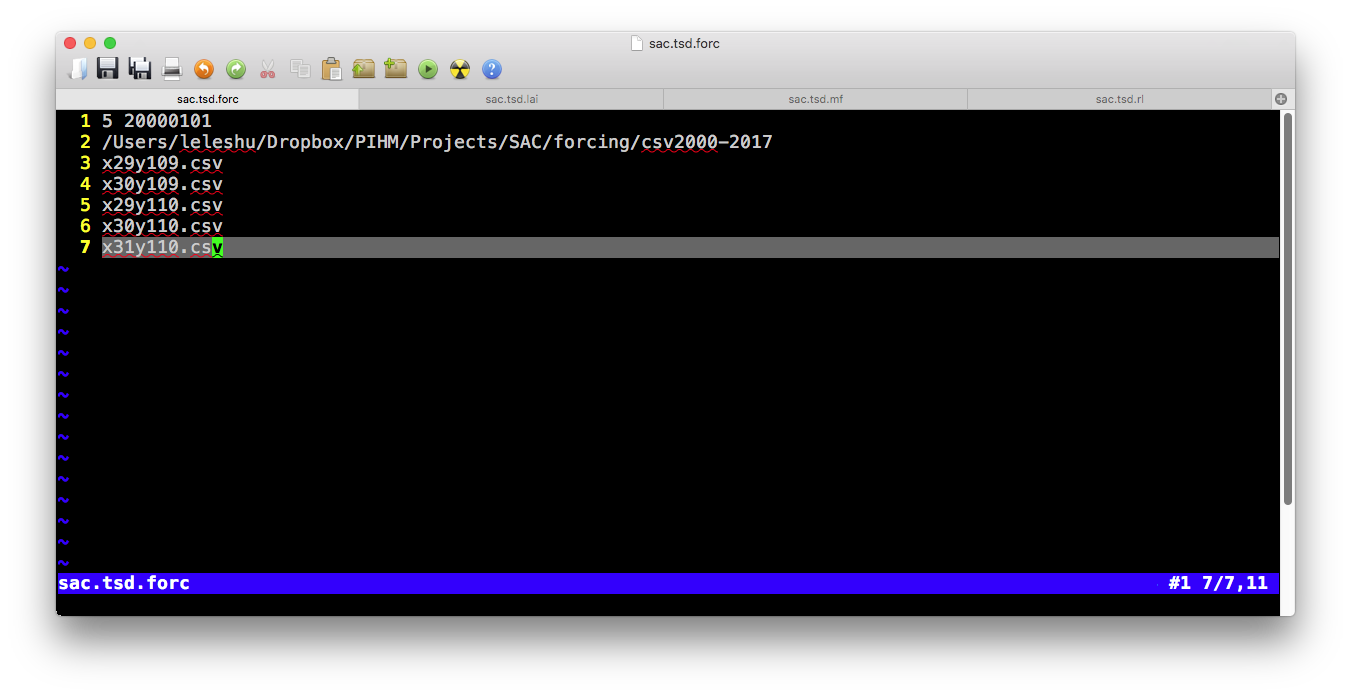
\includegraphics{Fig/IO/tsd.forc.png}
\caption{Example of .tsd.forc file}
\end{figure}

\begin{itemize}
\tightlist
\item
  Line 1:
  \texttt{Number\ of\ forcing\ sites\ \textbar{}\ Start\ day\ (YYYYMMDD)}
\item
  Line 2: Directory to the spreadsheet
\item
  Line 3\textasciitilde{}N: Filenames of spreadsheet
\end{itemize}

\begin{figure}
\centering
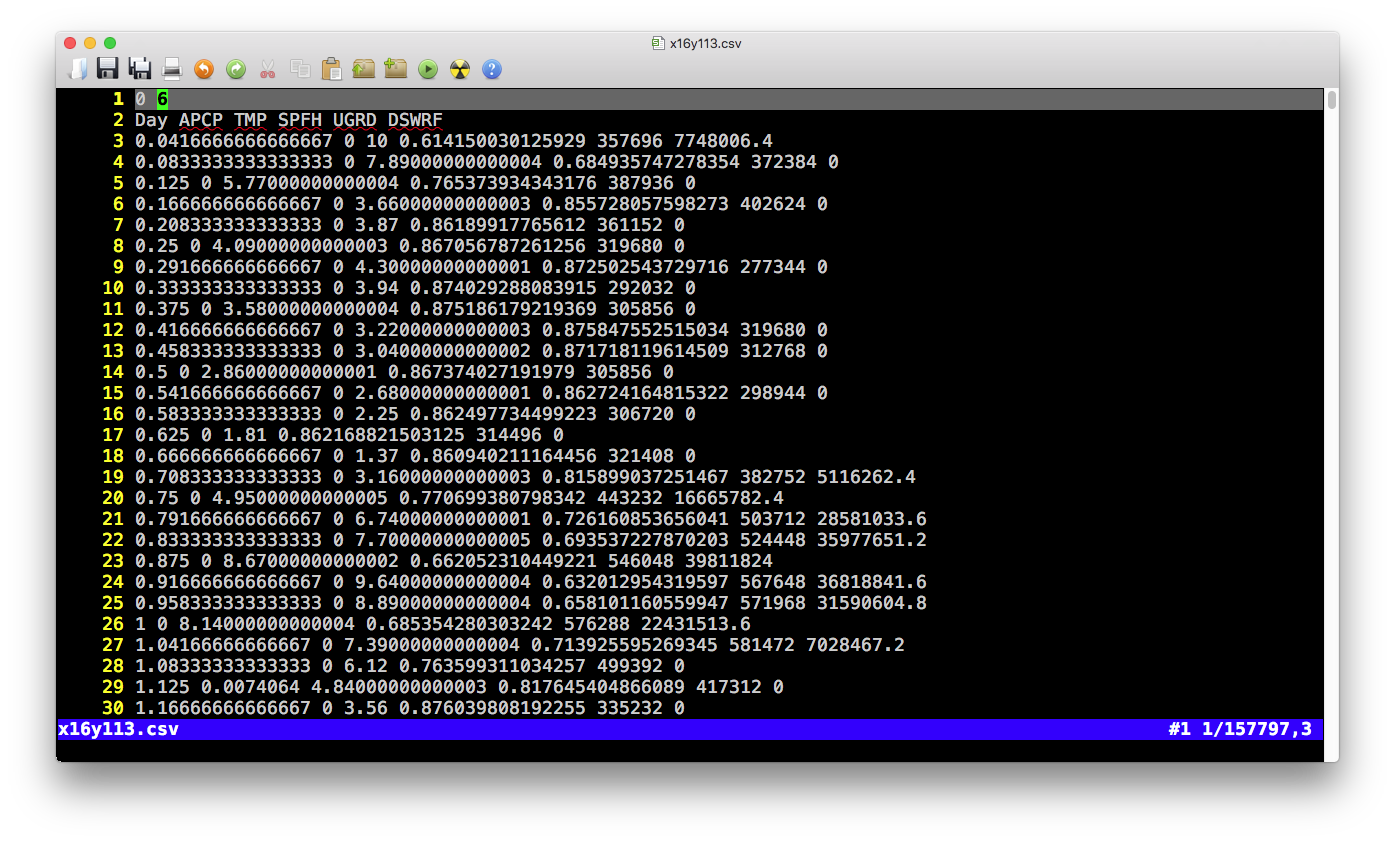
\includegraphics{Fig/IO/tsd.csv.png}
\caption{Example of .csv forcing file}
\end{figure}

\begin{itemize}
\tightlist
\item
  Pre-table:
\end{itemize}

\begin{longtable}[]{@{}cc@{}}
\toprule
Value1 & Value2\tabularnewline
\midrule
\endhead
( \(0\)) & Number of columns (\(6\))\tabularnewline
\bottomrule
\end{longtable}

\begin{itemize}
\tightlist
\item
  Table
\end{itemize}

\begin{longtable}[]{@{}ccccc@{}}
\toprule
Colname & Meaning & Range & Unit & Comments\tabularnewline
\midrule
\endhead
Day & Time & 0 \textasciitilde{} \(N_{day}\) & \(day\) &\tabularnewline
PRCP & Precipitation & 0 \textasciitilde{} 1 & \(m/day\)
&\tabularnewline
TEMP & Temperature & -100 \textasciitilde{} 70 & \(C\) &\tabularnewline
RH & Relative Humidity & 0 \textasciitilde{} 1 & \(-\) &\tabularnewline
wind & Wind Speed & 0 \textasciitilde{} inf & \(m/day\) &\tabularnewline
Rn & Solar (shortwave) radiation & ? & \(J/day/m^2\) &\tabularnewline
\bottomrule
\end{longtable}

\subsection{.tsd.lai file}\label{tsd.lai-file}

\begin{figure}
\centering
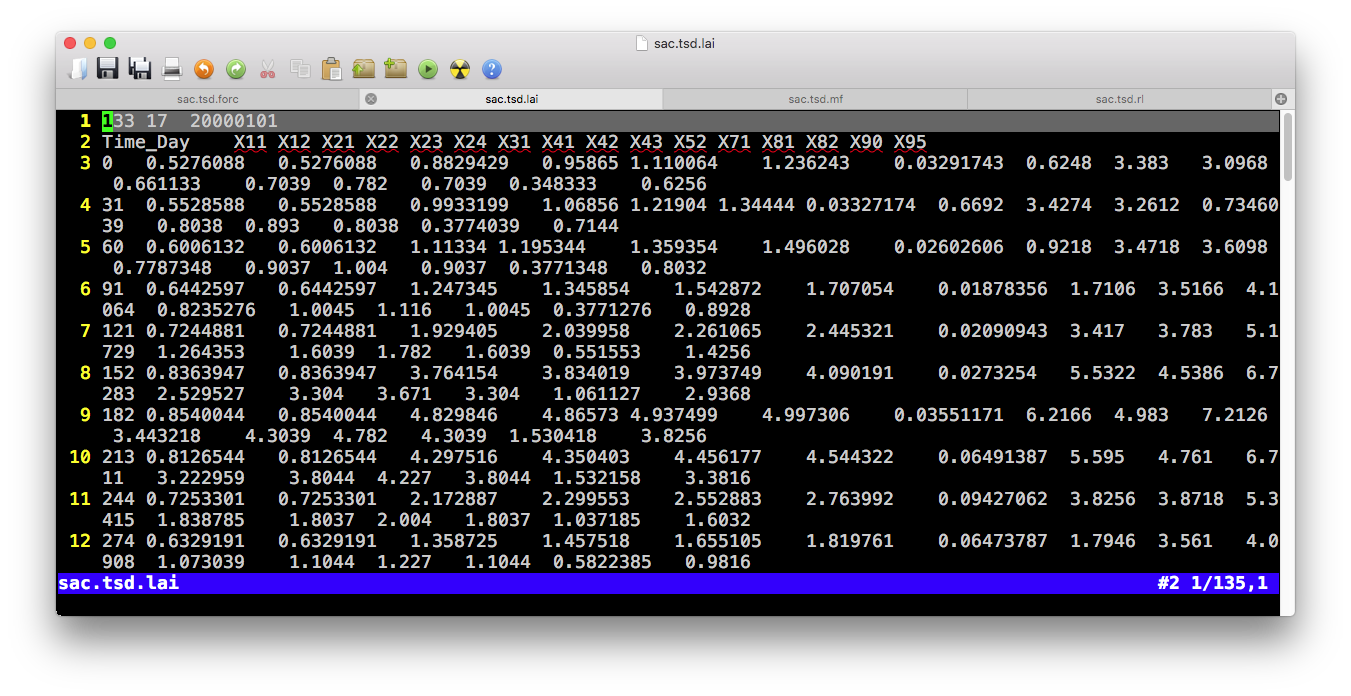
\includegraphics{Fig/IO/tsd.lai.png}
\caption{Example of .tsd.lai file}
\end{figure}

\begin{itemize}
\tightlist
\item
  Pre-table:
\end{itemize}

\begin{longtable}[]{@{}ccc@{}}
\toprule
Value1 & Value2 & Value3\tabularnewline
\midrule
\endhead
Number of day ( \(N_{time}\)) & Number of columns (\(N_{lc}\)) & Start
day (YYYYMMDD)\tabularnewline
\bottomrule
\end{longtable}

\begin{itemize}
\tightlist
\item
  Table
\end{itemize}

\begin{longtable}[]{@{}ccccc@{}}
\toprule
Colname & Meaning & Range & Unit & Comments\tabularnewline
\midrule
\endhead
TIME & Time & 0 \textasciitilde{} \(N_{time}\) & \(day\)
&\tabularnewline
Column 2 & LAI of land cover 1 & 0 \textasciitilde{} inf & \(m^2/m^2\)
&\tabularnewline
Column i & LAI of land cover \(i-1\) & 0 \textasciitilde{} inf &
\(m^2/m^2\) &\tabularnewline
\ldots{} & \ldots{} & \ldots{} & \ldots{} &\tabularnewline
\bottomrule
\end{longtable}

\subsection{.tsd.rl file}\label{tsd.rl-file}

\begin{figure}
\centering
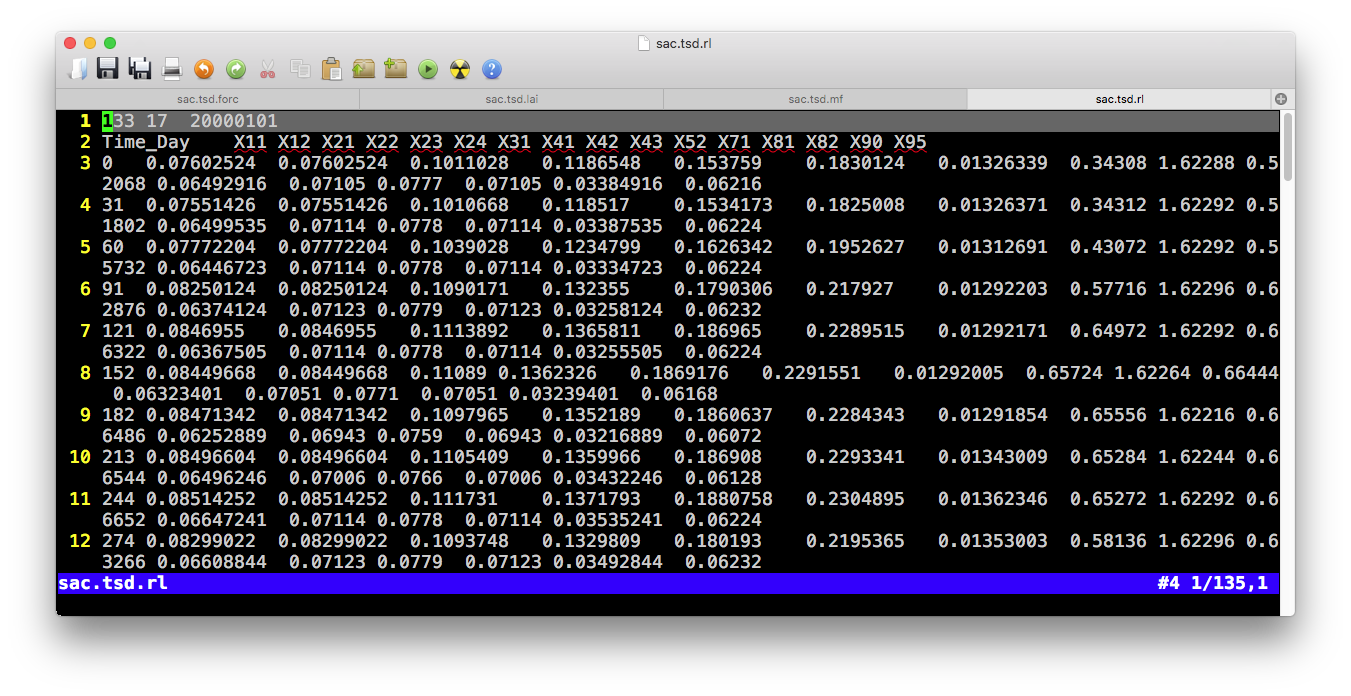
\includegraphics{Fig/IO/tsd.rl.png}
\caption{Example of .tsd.rl file}
\end{figure}

\begin{itemize}
\tightlist
\item
  Pre-table:
\end{itemize}

\begin{longtable}[]{@{}ccc@{}}
\toprule
Value1 & Value2 & Value3\tabularnewline
\midrule
\endhead
Number of day ( \(N_{time}\)) & Number of columns (\(N_{lc}\)) & Start
day (YYYYMMDD)\tabularnewline
\bottomrule
\end{longtable}

\begin{itemize}
\tightlist
\item
  Table
\end{itemize}

\begin{longtable}[]{@{}ccccc@{}}
\toprule
Colname & Meaning & Range & Unit & Comments\tabularnewline
\midrule
\endhead
TIME & Time & 0 \textasciitilde{} \(N_{time}\) & \(day\)
&\tabularnewline
Column 2 & Roughness length of land cover 1 & 0 \textasciitilde{} inf &
\(m\) &\tabularnewline
Column i & Roughness length of land cover \(i-1\) & 0 \textasciitilde{}
inf & \(m\) &\tabularnewline
\ldots{} & \ldots{} & \ldots{} & \ldots{} &\tabularnewline
\bottomrule
\end{longtable}

\subsection{.tsd.mf file}\label{tsd.mf-file}

\begin{figure}
\centering
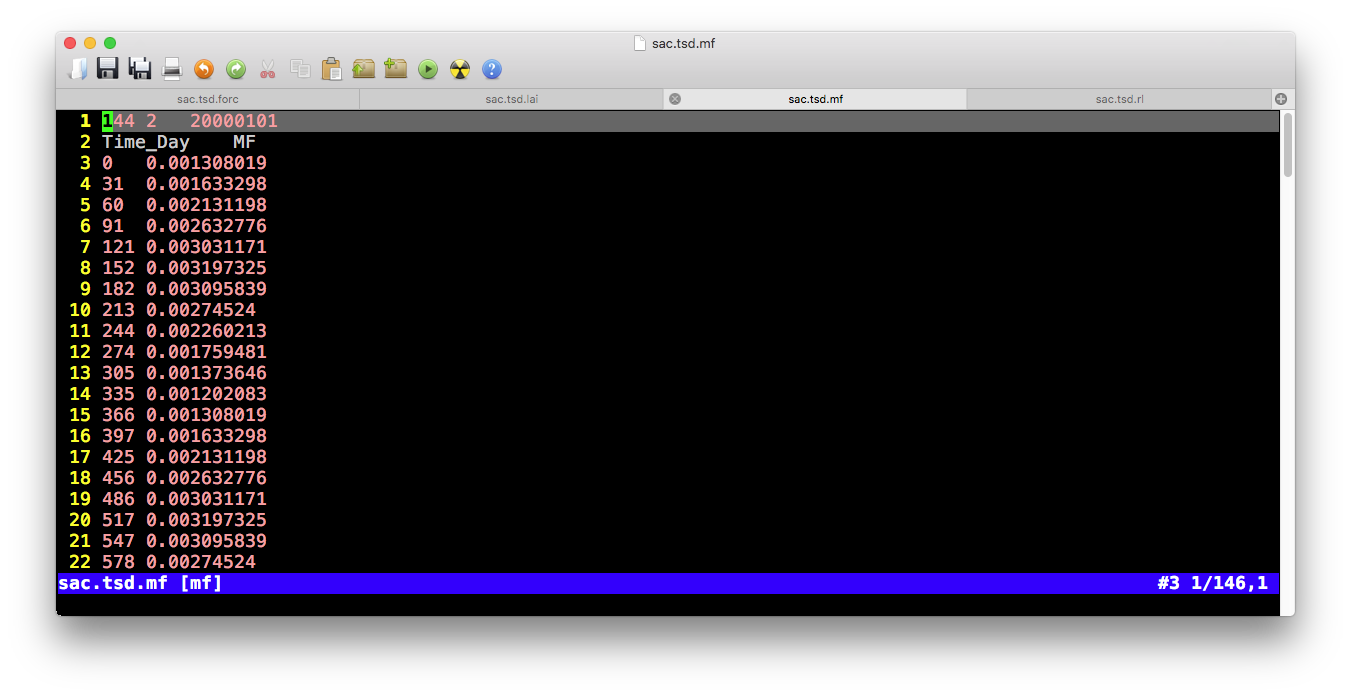
\includegraphics{Fig/IO/tsd.mf.png}
\caption{Example of .tsd.mf file}
\end{figure}

\begin{itemize}
\tightlist
\item
  Pre-table:
\end{itemize}

\begin{longtable}[]{@{}ccc@{}}
\toprule
Value1 & Value2 & Value3\tabularnewline
\midrule
\endhead
Number of day ( \(N_{time}\)) & Number of columns (\(N_{mf}\)) & Start
day (YYYYMMDD)\tabularnewline
\bottomrule
\end{longtable}

\begin{itemize}
\tightlist
\item
  Table
\end{itemize}

\begin{longtable}[]{@{}ccccc@{}}
\toprule
Colname & Meaning & Range & Unit & Comments\tabularnewline
\midrule
\endhead
TIME & Time & 0 \textasciitilde{} \(N_{time}\) & \(day\)
&\tabularnewline
Column 2 & Melt factor 1 & 0 \textasciitilde{} inf & - &\tabularnewline
Column i & Melt factor \(i-1\) & 0 \textasciitilde{} inf & -
&\tabularnewline
\ldots{} & \ldots{} & \ldots{} & \ldots{} &\tabularnewline
\bottomrule
\end{longtable}

\subsection{.tsd.obs file}\label{tsd.obs-file}

\begin{figure}
\centering
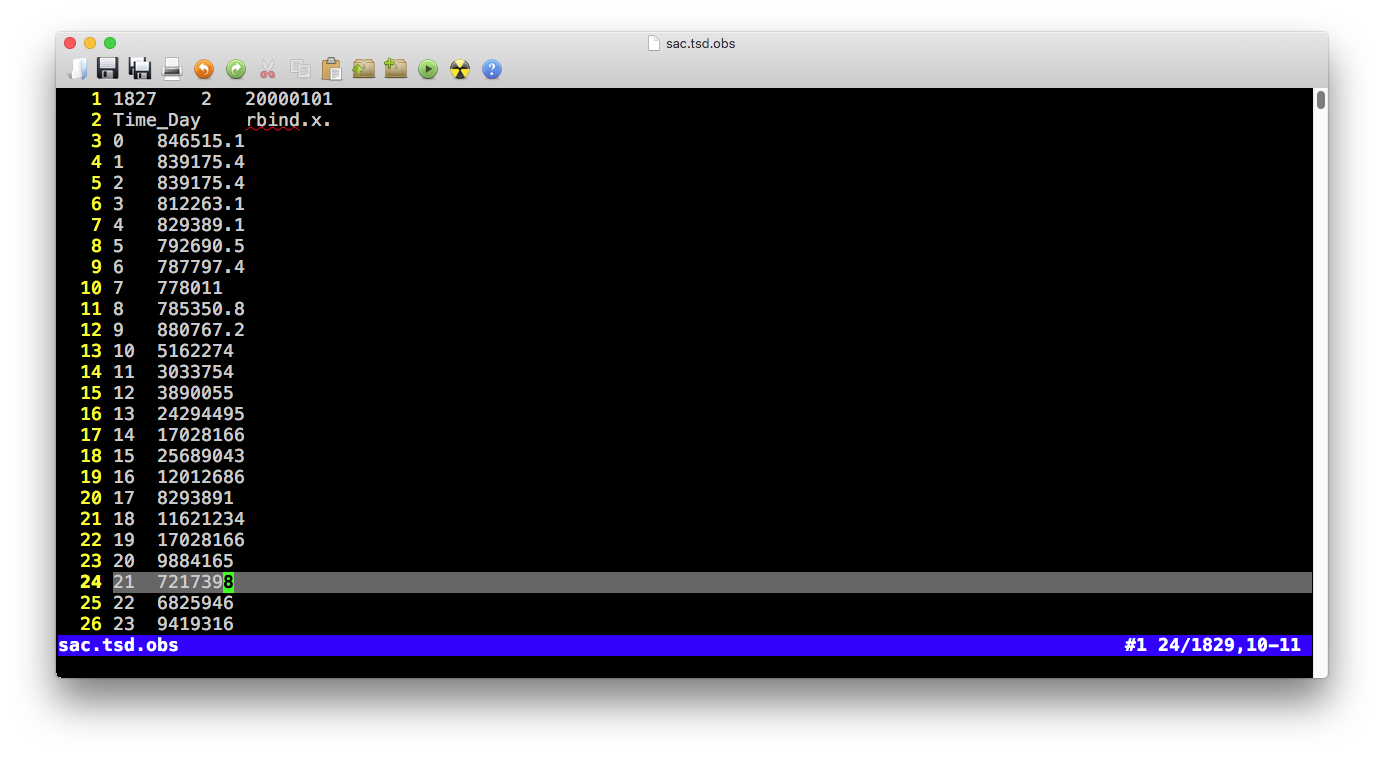
\includegraphics{Fig/IO/tsd.obs.png}
\caption{Example of .tsd.obs file}
\end{figure}

\begin{itemize}
\tightlist
\item
  Pre-table:
\end{itemize}

\begin{longtable}[]{@{}ccc@{}}
\toprule
Value1 & Value2 & Value3\tabularnewline
\midrule
\endhead
Number of day ( \(N_{time}\)) & Number of columns (\(N_{obs}\)) & Start
day (YYYYMMDD)\tabularnewline
\bottomrule
\end{longtable}

\begin{itemize}
\tightlist
\item
  Table
\end{itemize}

\begin{longtable}[]{@{}ccccc@{}}
\toprule
Colname & Meaning & Range & Unit & Comments\tabularnewline
\midrule
\endhead
TIME & Time & 0 \textasciitilde{} \(N_{time}\) & \(day\)
&\tabularnewline
Column 2 & Observational data 1 & ? & ? &\tabularnewline
Column i & Observational data \(i-1\) & ? & ? &\tabularnewline
\ldots{} & \ldots{} & \ldots{} & \ldots{} &\tabularnewline
\bottomrule
\end{longtable}

\chapter{Output files}\label{output-files}

\section{Output file names}\label{output-file-names}

Format of output file names:

\textbf{{[}Project Name{]}.{[}Identifier{]}.{[}Format{]}}

-The \emph{{[}Project Name{]}} is user defined name of the project, so
every input and output files must start with the \emph{{[}Project
Name{]}}. -The \emph{{[}Format{]}} is one of \emph{csv} or \emph{dat}.
\emph{csv} is spreadsheet format and \emph{dat} is bindary format.

The \emph{{[}Identifier{]}} is a combination of variables features, that
in format of: \textbf{{[}Model Unit{]}{[}Variable Type{]}{[}Variable
Name{]}}. \emph{{[}Model Unit{]}} is one of three options of \emph{ele}
(elemtns), \emph{riv} (river) or \emph{lak} (lake). Variable type
includes \emph{y}, \emph{v} and \emph{q} that are state variable (in
\(L\)), specific flux (in \(L^3/L^2/T\)) and flux (in \(L^3/T\))
respectively.

The list of output files is in following table.

\begin{longtable}[]{@{}ccccccc@{}}
\toprule
Identifier & Mod unit & Type & Var Name & Meaning & Unit\tabularnewline
\midrule
\endhead
\emph{.eleyic.} & ele & y & ic & Storage of Interception & \(m\)
&\tabularnewline
\emph{.eleysnow.} & ele & y & snow & Storage of snow equivalence & \(m\)
&\tabularnewline
\emph{.eleysurf.} & ele & y & surf & Storage of surface & \(m\)
&\tabularnewline
\emph{.eleyunsat.} & ele & y & unsat & Storage of vados zone & \(m\)
&\tabularnewline
\emph{.eleygw.} & ele & y & gw & Groundwater head & \(m\) &
.GW\tabularnewline
\emph{.elevetp.} & ele & v & etp & Potential ET & \(\frac{m^3}{m^2 d}\)
&\tabularnewline
\emph{.eleveta.} & ele & v & eta & Actual ET & \(\frac{m^3}{m^2 d}\)
&\tabularnewline
\emph{.elevetic.} & ele & v & etic & Evap of interception &
\(\frac{m^3}{m^2 d}\) &\tabularnewline
\emph{.elevettr.} & ele & v & ettr & Transpiration &
\(\frac{m^3}{m^2 d}\) &\tabularnewline
\emph{.elevetev.} & ele & v & etev & Soil Evaporation &
\(\frac{m^3}{m^2 d}\) &\tabularnewline
\emph{.elevprcp.} & ele & v & prcp & Precipitation &
\(\frac{m^3}{m^2 d}\) &\tabularnewline
\emph{.elevnetprcp.} & ele & v & netprcp & Net Precipitation &
\(\frac{m^3}{m^2 d}\) &\tabularnewline
\emph{.elevinfil.} & ele & v & infil & Infiltration Rate &
\(\frac{m^3}{m^2 d}\) &\tabularnewline
\emph{.elevexfil.} & ele & v & infil & Exfiltration Rate &
\(\frac{m^3}{m^2 d}\) &\tabularnewline
\emph{.elevrech.} & ele & v & rech & Recharge Rate &
\(\frac{m^3}{m^2 d}\) &\tabularnewline
\emph{.eleqsurf.} & ele & q & surf & Overland flow & \(m^3/d\)
&\tabularnewline
\emph{.eleqsub.} & ele & q & sub & Subsurface flow & \(m^3/d\)
&\tabularnewline
\emph{.rivystage.} & riv & y & stage & River Stage & \(m\)
&\tabularnewline
\emph{.rivqup.} & riv & q & up & Flux to upstream & \(m^3/d\)
&\tabularnewline
\emph{.rivqdown.} & riv & q & down & Flux to downstream & \(m^3/d\)
&\tabularnewline
\emph{.rivqsurf.} & riv & q & surf & Flux to landsurface & \(m^3/d\)
&\tabularnewline
\emph{.rivqsub.} & riv & q & sub & Flux to subsurface & \(m^3/d\)
&\tabularnewline
\bottomrule
\end{longtable}

\section{Data format in ASCII (.csv)
file}\label{data-format-in-ascii-.csv-file}

N - Number of column of output data, excluding the time column. m -
Number of time-step. StartTime - String of date/time (YYYYMMDD or
YYYYMMDD.hhmmss)

\begin{longtable}[]{@{}cccccc@{}}
\toprule
N & StartTime & & & &\tabularnewline
\midrule
\endhead
\(T_1\) & \(v_{1 \cdot 1}\) & \(v_{1 \cdot 2}\) & \ldots{} &
\(v_{1 \cdot N}\) &\tabularnewline
\(T_2\) & \(v_{2 \cdot 1}\) & \(v_{2 \cdot 2}\) & \ldots{} &
\(v_{2 \cdot N}\) &\tabularnewline
\(T_3\) & \(v_{3 \cdot 1}\) & \(v_{3 \cdot 2}\) & \ldots{} &
\(v_{3 \cdot N}\) &\tabularnewline
\ldots{} & \ldots{} & \ldots{} & \ldots{} & \ldots{} &\tabularnewline
\(T_{m}\) & \(v_{m \cdot 1}\) & \(v_{m \cdot 2}\) & \ldots{} &
\(v_{m \cdot N}\) &\tabularnewline
\bottomrule
\end{longtable}

\section{Data format in binary (.dat)
file}\label{data-format-in-binary-.dat-file}

The value saved in binary file are identical from ASCII format, but
different data structure.

\begin{longtable}[]{@{}ccccc@{}}
\toprule
ID & \(i\) & Value & Format & Length\tabularnewline
\midrule
\endhead
1 & - & \(N\) & double & 8\tabularnewline
2 & - & StartTime & double & 8\tabularnewline
3 & 0 & \(T_1\) & double & 8\tabularnewline
4 & 1 & \(v_{1 \cdot 1}\) & double & 8\tabularnewline
5 & 2 & \(v_{1 \cdot 2}\) & double & 8\tabularnewline
\ldots{} & \ldots{} & \ldots{} & double & 8\tabularnewline
\((N+1) * (T-1) + i +3\) & N & \(v_{1 \cdot N}\) & double &
8\tabularnewline
\((N+1) * (T-1) + i +3\) & 0 & \(T_2\) & double & 8\tabularnewline
\((N+1) * (T-1) + i +3\) & 1 & \(v_{2 \cdot 1}\) & double &
8\tabularnewline
\((N+1) * (T-1) + i +3\) & 2 & \(v_{2 \cdot 2}\) & double &
8\tabularnewline
\((N+1) * (T-1) + i +3\) & \ldots{} & \ldots{} & double &
8\tabularnewline
\((N+1) * (T-1) + i +3\) & N & \(v_{2 \cdot N}\) & double &
8\tabularnewline
\((N+1) * (T-1) + i +3\) & 0 & \(T_3\) & double & 8\tabularnewline
\((N+1) * (T-1) + i +3\) & 1 & \(v_{3 \cdot 1}\) & double &
8\tabularnewline
\((N+1) * (T-1) + i +3\) & 2 & \(v_{3 \cdot 2}\) & double &
8\tabularnewline
\((N+1) * (T-1) + i +3\) & \ldots{} & \ldots{} & double &
8\tabularnewline
\((N+1) * (T-1) + i +3\) & N & \(v_{3 \cdot N}\) & double &
8\tabularnewline
\((N+1) * (T-1) + i +3\) & \ldots{} & \ldots{} & double &
8\tabularnewline
\((N+1) * (T-1) + i +3\) & \ldots{} & \ldots{} & double &
8\tabularnewline
\((N+1) * (T-1) + i +3\) & \ldots{} & \ldots{} & double &
8\tabularnewline
\((N+1) * (T-1) + i +3\) & \ldots{} & \ldots{} & double &
8\tabularnewline
\((N+1) * (m-1) + i +3\) & 0 & \(T_{m}\) & double & 8\tabularnewline
\((N+1) * (m-1) + i +3\) & 1 & \(v_{m \cdot 1}\) & double &
8\tabularnewline
\((N+1) * (m-1) + i +3\) & 2 & \(v_{m \cdot 2}\) & double &
8\tabularnewline
\((N+1) * (m-1) + i +3\) & \ldots{} & \ldots{} & double &
8\tabularnewline
\((N+1) * (m-1) + i +3\) & N & \(v_{m \cdot N}\) & double &
8\tabularnewline
\bottomrule
\end{longtable}

\chapter{Applications}\label{applications}

Some \emph{significant} applications are demonstrated in this chapter.

\section{Best practice suggestions}\label{best-practice-suggestions}

\begin{enumerate}
\def\labelenumi{\arabic{enumi}.}
\tightlist
\item
  Derive and QC all inputs (time mean, accumulation, screen fo
  anormalies \ldots{})
\item
  Conduct offline simulations \ldots{}
\item
  Start with `idealized' forcing (Option FORC\_debug=1 in .cfg.para
  file). Which will use uniform forcing data to drive the hydrologic
  simulations.
\item
  Run with short time period, load the outputs and examine whether
  results are in expection
\item
  If all above works, then hook all modules and run with your forcing
  data.
\end{enumerate}

\emph{This chapter is imcomplete}

\section{Example 1: Vauclin
Experiment}\label{example-1-vauclin-experiment}

\section{Example 2: Shall Hill CZO}\label{example-2-shall-hill-czo}

\section{Example 3: Conestoga Watershed,
Pennsylvanis}\label{example-3-conestoga-watershed-pennsylvanis}

\chapter{Calibration}\label{calibration}

\emph{This chapter is imcomplete}

\begin{longtable}[]{@{}cccc@{}}
\toprule
File & Comments & Header & \# of column\tabularnewline
\midrule
\endhead
.cfg.cmaes & Configuration of CMA-ES method & No & -\tabularnewline
\bottomrule
\end{longtable}

Values in .calib.cmaes file:

\begin{longtable}[]{@{}ccccc@{}}
\toprule
Item & Meaning & Default value & Range & Unit\tabularnewline
\midrule
\endhead
lambda & Number of children in each generation & 48 & & -\tabularnewline
stopfitness & Threshold to accept the \emph{best} solution & 0.3 & &
-\tabularnewline
maxgen & Maximun generations & 48 & & -\tabularnewline
sigma & & 0.8 & & -\tabularnewline
updateic & Whether to update initial condition after each generation & 0
& 0/1 & -\tabularnewline
walltime & Walltime to kill the modeling thread & 86400 & 0-inf &
second\tabularnewline
nspingup & Number of days for spinup & 0 & 0-inf & day\tabularnewline
& & & & -\tabularnewline
\bottomrule
\end{longtable}

Values in .calib.range file:

Rows: Values in .cfg.calib file. Column: \textbar{} Item \textbar{}
Meaning \textbar{} Default value \textbar{} Range \textbar{} Unit
\textbar{}
\textbar{}:------:\textbar{}:--------------------------:\textbar{}:---------:\textbar{}:---------:\textbar{}:--------:\textbar{}
\textbar{} On/off \textbar{} On or Off \textbar{} 0 \textbar{} 0/1
\textbar{} - \textbar{} \textbar{} log \textbar{} Whether logrithm
\textbar{} 0 \textbar{} 0/1 \textbar{} - \textbar{} \textbar{} min
\textbar{} Minimun value \textbar{} - \textbar{} - \textbar{} -
\textbar{} \textbar{} max \textbar{} Maximun value \textbar{} -
\textbar{} - \textbar{} - \textbar{}

\chapter{Quick, Reproducible and Automatic hydrological
modeling}\label{quick-reproducible-and-automatic-hydrological-modeling}

Automatic deployment of SHUD System

\chapter{Source code and program
design}\label{source-code-and-program-design}

The source code of SHUD and SHUD-tool are avaliable via Github:
\url{https://github.com/SHUD-System/SHUD} and
\url{https://github.com/SHUD-System/SHUD-tools}.

\bibliography{book.bib}

\end{document}
